\documentclass[spanish]{article}
\usepackage{titlesec}

%Quitar páginas en blanco
\let\cleardoublepage\clearpage
\usepackage{etoolbox}
\makeatletter
\patchcmd{\@endpart}{\vfil\newpage}{\par}{}{}
\makeatother

%\usepackage[spanish]{babel} ¡Esto estaba interfiriendo con las flechitas de los \tikspicture

\usepackage[left=4cm, right=4cm]{geometry}
\usepackage{palatino}%Font
\usepackage{graphicx}
\usepackage{wrapfig}
\usepackage{marvosym}%Smileys
\usepackage{float}
\usepackage{subcaption}
\usepackage[shortlabels]{enumitem}
\usepackage{parskip}
\usepackage{amsthm}
\usepackage{amssymb}
\usepackage{amsmath}
\usepackage{mathtools}
\usepackage{stmaryrd}
\usepackage{pst-solides3d}
\usepackage{tikz}
\usepackage{tikz-cd}
\usetikzlibrary{shapes.geometric}
\usetikzlibrary{%
	matrix,%
	calc,%
	arrows,%
	shapes,
	decorations,
	decorations.markings
}
\usetikzlibrary{arrows, arrows.meta}
\usepackage[bookmarks,bookmarksopen,bookmarksdepth=3]{hyperref}
\hypersetup{
	colorlinks=true,
	urlcolor=blue,
	linkcolor=magenta,
	citecolor=blue,
	filecolor=blue,
	urlbordercolor=white,
	linkbordercolor=white,
	citebordercolor=white,
	filebordercolor=white
}

\theoremstyle{definition}
\renewcommand{\proofname}{Demostración}

\newtheorem*{defn}{Definición}
\newtheorem*{lema}{Lema}
\newtheorem*{obs}{Observación}
\newtheorem*{teo}{Teorema}
\newtheorem*{prop}{Proposición}
\newtheorem*{coro}{Corolario}
\newtheorem*{af}{Afirmación}
\newtheorem*{ejer}{Ejercicio}
\newtheorem*{ejem}{Ejemplo}
\newtheorem*{pregunta}{Pregunta}

\newcommand{\R}{\mathbb{R}}
\newcommand{\Z}{\mathbb{Z}}
\newcommand{\N}{\mathbb{N}}
\newcommand{\C}{\mathbb{C}}
\newcommand{\Q}{\mathbb{Q}}
\newcommand{\Hy}{\mathbb{H}}
\newcommand{\A}{\mathbb{A}}
\newcommand{\D}{\mathbb{D}}
\newcommand{\M}{\mathbb{M}}
\DeclareMathOperator{\Id}{Id}
\DeclareMathOperator{\img}{img}
\DeclareMathOperator{\rel}{rel}
\DeclareMathOperator{\Mod}{Mod}
\DeclareMathOperator{\Hom}{Hom}
\DeclareMathOperator{\Homeo}{Homeo}
\DeclareMathOperator{\Isom}{Isom}
\DeclareMathOperator{\Deck}{Deck}
\DeclareMathOperator{\Diff}{Diff}
\DeclareMathOperator{\SL}{SL}
\DeclareMathOperator{\PSL}{PSL}
\DeclareMathOperator{\SMod}{SMod}
\DeclareMathOperator{\LMod}{LMod}
\DeclareMathOperator{\PMod}{PMod}
\DeclareMathOperator{\SHomeo}{\mathcal{S}Homeo}
\DeclareMathOperator{\LHomeo}{\mathcal{L}Homeo}

\usepackage[backend=bibtex]{biblatex}
\addbibresource{expo-bir.bib}

\renewcommand{\contentsname}{}
\title{Aplicaciones a presentaciones del grupo modular}
\date{}
\author{Daniel González Casanova Azuela}

\begin{document}
	\maketitle
	\vspace{-2cm}
%	\phantomsection
%	\addcontentsline{toc}{part}{\contentsname}
	\tableofcontents
\section{Preliminares}
\subsection{Definiciones}
Comenzamos revisando los conceptos fundamentales. (Las definiciones se pueden omitir en la exposición)

	\begin{enumerate}
		\item El \textbf{\textit{mapping class group}} $\Mod(S_{g,n})$ de una superficie cerrada, orientable de género $g$ con $n$ puntos marcados $S_{g,n}$ es el grupo de clases de homotopía de homeomorfismos que preservan la orientación, la frontera y el conjunto de puntos marcados. (Las homotopías también preservan la frontera y los puntos marcados.)
		
		\item Una función $p:S\to X$ es un \textbf{\textit{cubriente ramificado}} si existe un conjunto finito $B\subseteq X$ tal que la restricción $S\backslash p^{-1}(B)\to X\backslash B$ es un cubriente. El \textbf{\textit{grado}}  de $p$ es $d$ si el grado del cubriente asociado es $d$. Los \textbf{\textit{puntos de ramificación}} son puntos con menos preimágenes que $d$. Decimos que $p$ es \textbf{\textit{regular}} si el grupo de transformaciones de cubierta actúa transitivamente en $S$.
		
		\item Decimos que un grupo finito $G$ es \textbf{\textit{soluble}} si tiene una \textbf{\textit{serie normal}}
		\[G=G_0\geq G_1\geq G_2\geq\cdots\geq G_t=\{1\}\]
		cuyos \textbf{\textit{grupos factores}}
		\[G_0/G_1,G_1/G_2,\ldots,G_{n-1}/G_n\]
		son abelianos (\cite{Rotman}, prop. 5.59).
		
		\item El grupo de \textbf{\textit{transformaciones de cubierta}} de un cubriente $p$ es ${\operatorname{Deck}(p)=\{h:S\overset{\text{homeo}}{\longrightarrow} S\;|p=hp\}}$.
		\[\begin{tikzcd}[column sep=tiny]
			S\arrow[rr,"h"]\arrow[rd,"p",swap]&&S\arrow[ld,"p"]\\
			&X
		\end{tikzcd}\]
		Decimos que $p$ es un \textbf{\textit{cubriente soluble}} si $\Deck(p)$ es soluble.
		
		\item Un homeomorfismo $f:X\to X$ se \textbf{\textit{levanta}} a $\tilde{f}:S\to S$ si $p\tilde{f}= pf$ para cualquier punto de $S$.
		\[\begin{tikzcd}
			S\arrow[r,"\tilde{f}"]\arrow[d,"p",swap]&S\arrow[d,"p"]\\
			X\arrow[swap,r,"f"]&X
		\end{tikzcd}\]
		
		$\LMod(X)$ es el subgrupo de clases de equivalencia en $\Mod(X)$ que tienen un representante que se levanta a $S$. (Recordemos que $fp$ se levanta a $\tilde{f}$ si y sólo si $(fp)_*\pi_1(S)\subset p_*\pi_1(S)$.)
		
		\item Una función $\tilde{f}:S\to S$ \textbf{\textit{preserva fibras}} si para cualquier $x\in X$ existe $y\in X$ tal que $\tilde{f}(p^{-1}(x))=p^{-1}(y)$ como conjuntos, es decir, $\tilde{f}$ manda fibras en fibras.
		
		$\SMod(S)$ es el subgrupo de clases de equivalencia en $\Mod(S)$ que tienen un representante que preserva fibras (la homotopía puede no preservar fibras). Son exactamente los levantamientos de los homeomorfismos levantables.
		
		\item El \textbf{\textit{mapping class group puro $\PMod(S_{g,n})$}} es el subgrupo de $\Mod(S_{g,n})$ consiste de los elementos que fijan cada punto marcado individualmente.
		
		\item Decimos que $p$ tiene la \textbf{\textit{propiedad de Birman-Hilden}} si para cualesquiera dos homeomorfismos homotópicos que preservan fibras hay una homotopía entre ellos que preserva fibras.
		
	\end{enumerate}

La idea de la teoría de Birman-Hilden es estudiar el mapping class group del cociente mediante el mapping class group del cubriente. Para esto necesitamos que una homotopía del cubriente preserve fibras, ya que sólo este caso desciende al cociente.

\subsection{Resultados que usaremos}

\subsubsection{Teorema de Birman-Hilden y equivalencias}

\begin{teo}[Birman-Hilden]
	Sea $p:S\to X$ un cubriente regular ramificado con un número finito de hojas donde $S$ es una superficie hiperbólica. Supongamos que $p$ o bien no es ramificado o bien es soluble. Entonces $p$ tiene la propiedad de Birman-Hilden.
\end{teo}
\begin{prop}
	Sea $p:S\to X$ un cubriente regular ramificado con un número finito de hojas donde $S$ es una superficie hiperbólica sin frontera. Las siguientes son equivalentes:
	\begin{enumerate}[(i)]
		\item $p$ tiene la propiedad de Birman-Hilden.
		\item El mapeo natural $\LMod(X)\to\SMod/D$ es inyectivo.
		\item El mapeo natural $\SMod(S)\to\LMod(X)$ está bien definido.
		\item $\SMod(S)/D\cong\LMod(X)$.
	\end{enumerate}
	donde $D$ son las clases de homotopía de transformaciones de cubierta de $S$.
\end{prop}
\begin{proof}
	Primero simplemente observemos que el mapeo $\LMod(X)\to\SMod(S)$ siempre está bien definido por la propiedad del levantamiento de homotopías:
	\[\begin{tikzcd}[ampersand replacement=\&]
		\&\& S\arrow[d,"p"]\\
		S\arrow[dashed,urr,"\widetilde{fp}\simeq\widetilde{gp}"]\arrow[r,swap,"p"]\& X\arrow[r,swap,"f\simeq g"]\& X
	\end{tikzcd}\]
	
	Observemos también que las transformaciones de cubierta son levantamientos de la identidad.
	\[\begin{tikzcd}[ampersand replacement=\&]
		\&\& S\arrow[d,"p"]\\
		S\arrow[dashed,urr,"\widetilde{\Id}"]\arrow[r,swap,"p"]\& X\arrow[r,swap,"\Id"]\& X
	\end{tikzcd}\]
	
	(i)$\implies$(ii) Tomamos el neutro en $\SMod(S)/D$ y mostramos que su única preimagen es el neutro en $\LMod(X)$. En efecto, si $\widetilde{fp}\simeq\tilde{\Id}$, por (i) la homotopía preserva fibras, desciende al cociente y obtenemos que $f\simeq \Id$.
	
	\[\begin{tikzcd}[ampersand replacement=\&]
		\&\& S\arrow[d,"p"]\\
		S\arrow[dashed,urr,"\widetilde{fp}\simeq\widetilde{\Id}"]\arrow[r,swap,"p"]\& X\arrow[r,swap,"f\simeq\Id"]\& X
	\end{tikzcd}\]
	
	(ii)$\implies$(iii) En el siguiente diagrama
	\[\begin{tikzcd}[ampersand replacement=\&]
		\&\SMod(S)\arrow[d,"\pi"]\arrow[ld,dashed]\\
		\LMod(X)\arrow[r,leftrightarrow,swap,"\text{(ii)}"]\&\SMod(S)/D
	\end{tikzcd}\]
	la flecha punteada es el mapeo natural.
	
	(iii)$\implies$(i)  Supongamos que  $\widetilde{fp}\simeq\widetilde{gp}$ y veamos que hay una homotopía que preserva fibras. Por (iii), $\widetilde{f}\simeq\widetilde{g}$, y por la propiedad del levantamiento terminamos.
	
	\[\begin{tikzcd}[ampersand replacement=\&]
		\&\& S\arrow[d,"p"]\\
		S\arrow[dashed,urr,"\widetilde{fp}\simeq\widetilde{gp}"]\arrow[r,swap,"p"]\& X\arrow[r,swap,"f\simeq g"]\& X
	\end{tikzcd}\]
	
	(ii)$\implies $(iv) Primer teorema de isomorfismo.
\end{proof}


%Pensemos rápidamente en cómo está definido el mapeo natural $\LMod(X)\to\SMod$ tomando la clase de homotopía identidad en $\LMod(X)$. Cuando levantamos cualquier representante de la clase, existe un único levantamiento de cada función en la homotopía, de manera que tenemos un elemento en $\SMod(\tilde{X})$.

%El detalle es que nada nos asegura que las funciones de en medio preserven fibras, ya que, por definición, sólo el representante de la clase es levantable.

%Cuando tomamos la clase de equivalencia de una transformación de deck, si no tenemos la propiedad de Birman-Hilden, no podemos construir una homotopía con la identidad en el cociente.

\subsubsection{Generadores de $\Mod(S_g)$}

\begin{teo}[Generadores de Humphries (\cite{primer}, teo. 4.14)]
	Si $g\geq2$, entonces $\Mod(S_g)$ está generado por los giros de Dehn respecto a las $2g+1$ clases de isotopía de las curvas simples, cerradas y no separantes mostradas en la siguiente figura:
	\begin{figure}[H]
		\centering
		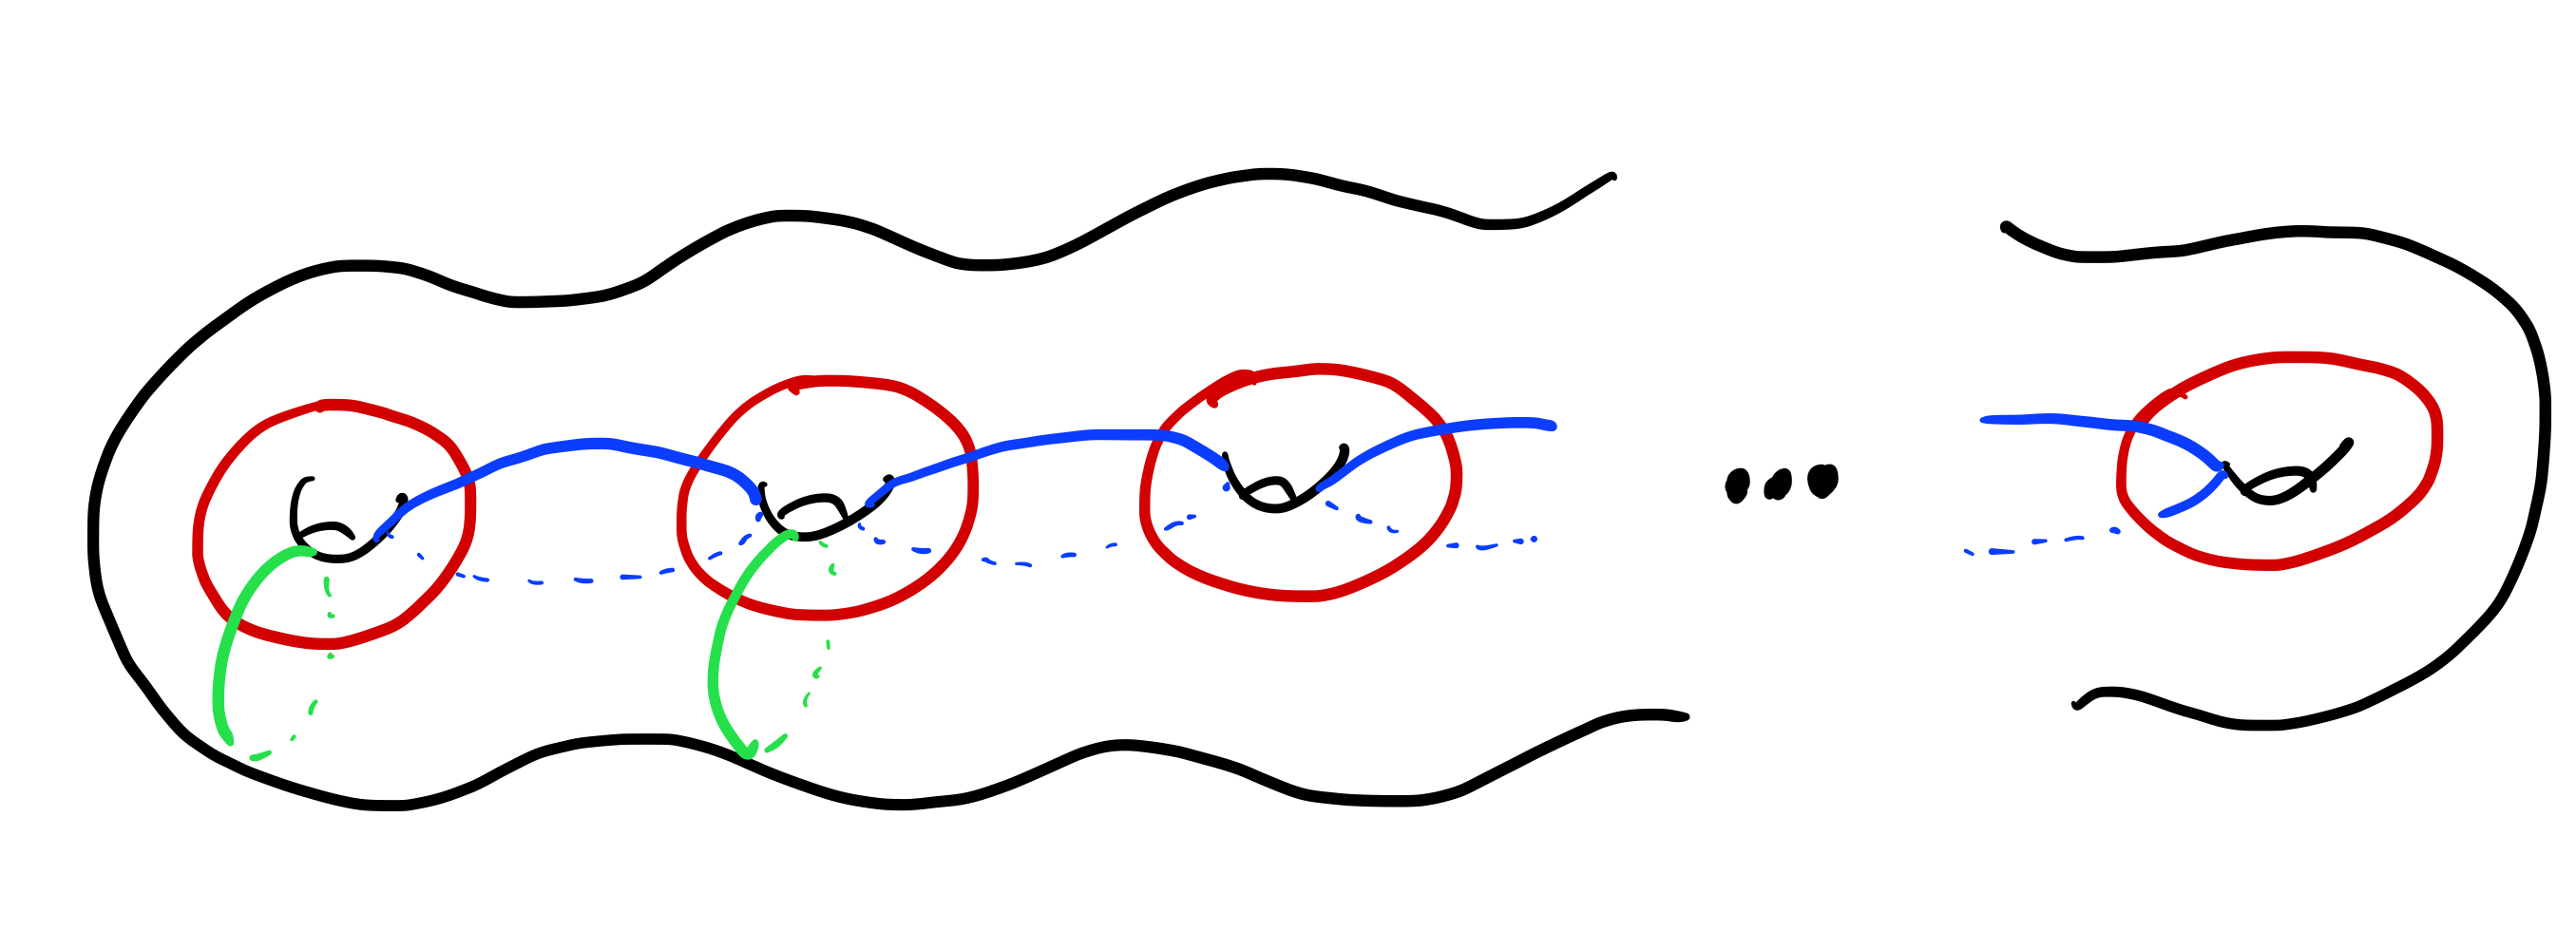
\includegraphics[width=0.9\linewidth]{fig0}
	\end{figure}
\end{teo}

Recordemos que los giros de Dehn actúan de la siguiente forma. Tomando como ejemplo una de las curvas verdes y una vecindad suya con una curva naranja de referencia,

	\begin{figure}[H]
	\centering
	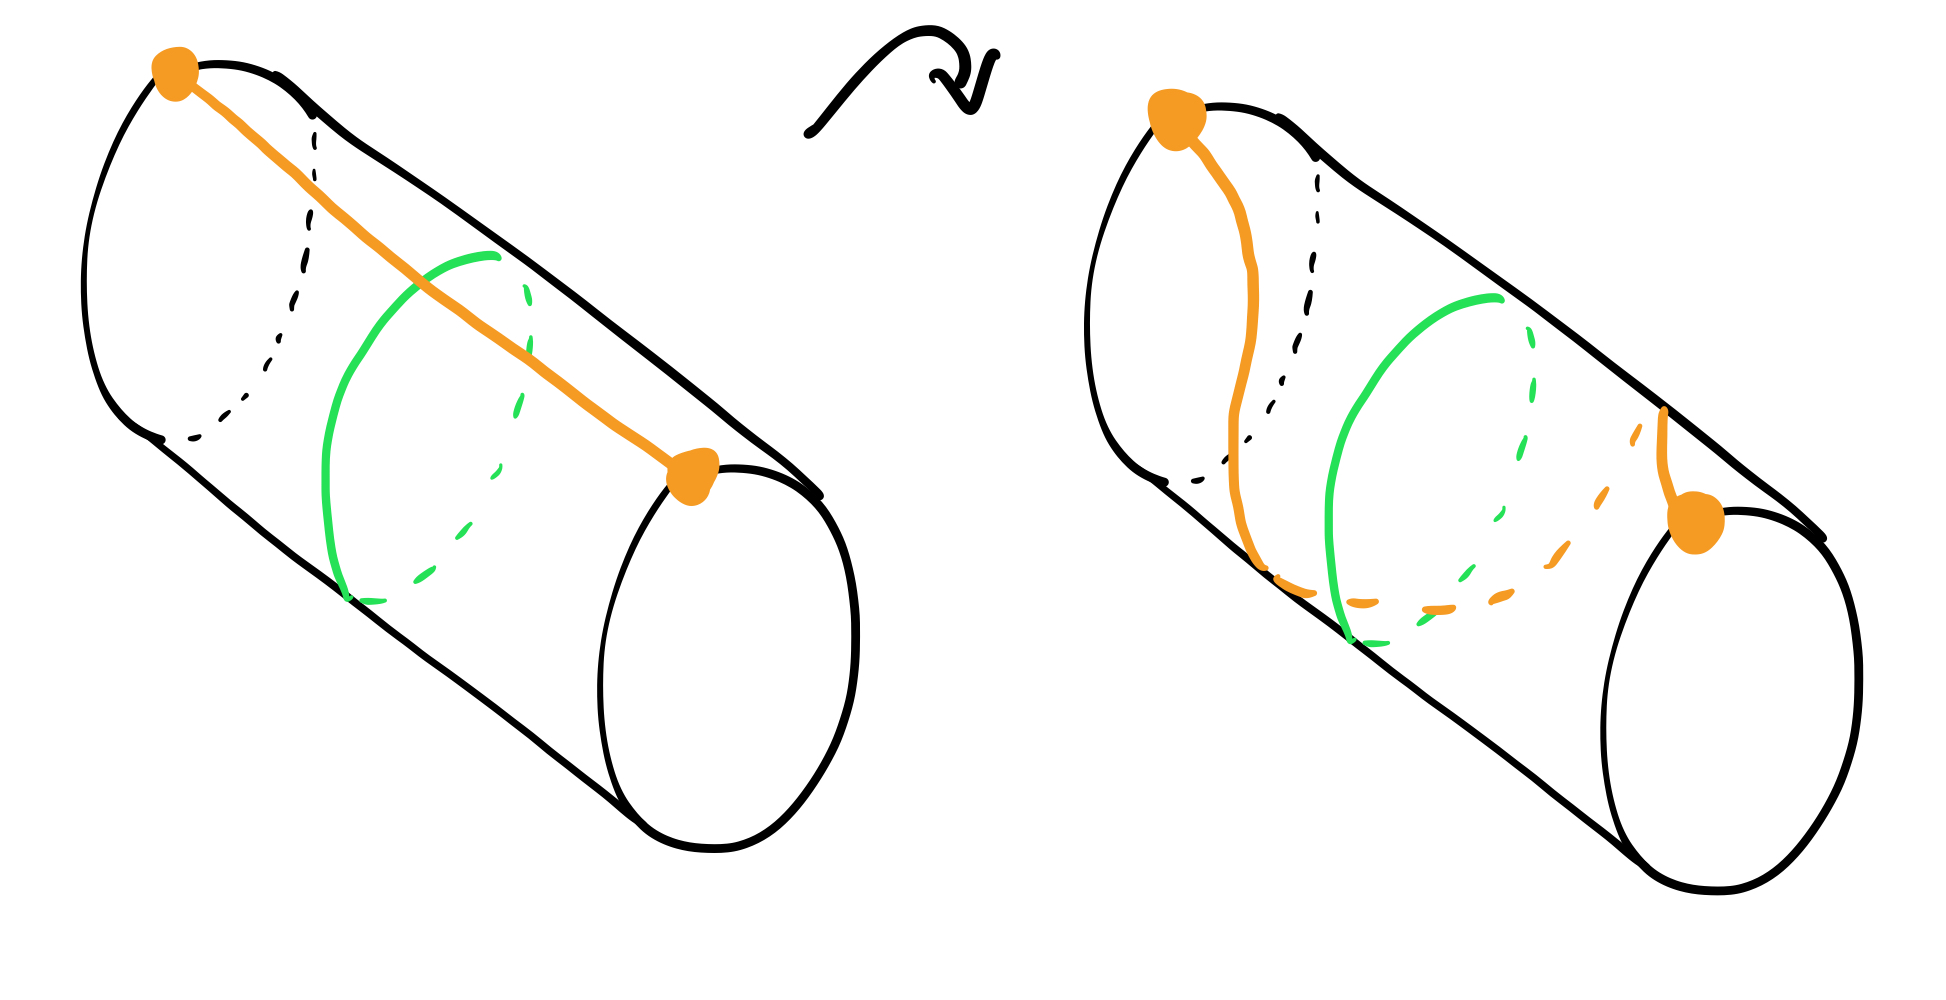
\includegraphics[width=0.7\linewidth]{fig0p}
\end{figure}

\subsubsection{Generadores de $\Mod(S_{0,n})$}

Para el caso de la esfera con puntos marcados, consideremos la siguiente sucesión exacta:
\[\begin{tikzcd}
	1\arrow[r]&\PMod(S_{0,n})\arrow[hook,r]&\Mod(S_{0,n})\arrow[r,two heads]&\Sigma_n\arrow[r]&1
\end{tikzcd}\]
donde la flecha inyectiva es la inclusión y la suprayectiva es la acción de cada homeomorfismo de $S_{0,n}$ en la colección de puntos marcados vista como una permutación ($\Sigma_n$ es el grupo de permutaciones de $n$ elementos).

Esta sucesión exacta implica que
\[\frac{\Mod(S_{0,n})}{\PMod(S_{0,n})}\approx\Sigma_n\]
Por lo tanto, este cociente está generado por los levantamientos de una colección de generadores de $\Sigma_n$. Es natural escoger las transposiciones para generar el grupo de permutaciones, que se levantan a mapping classes como mostramos a continuación.

Tomemos el ejemplo de un disco con tres puntos marcados:
\begin{figure}[H]
	\centering
	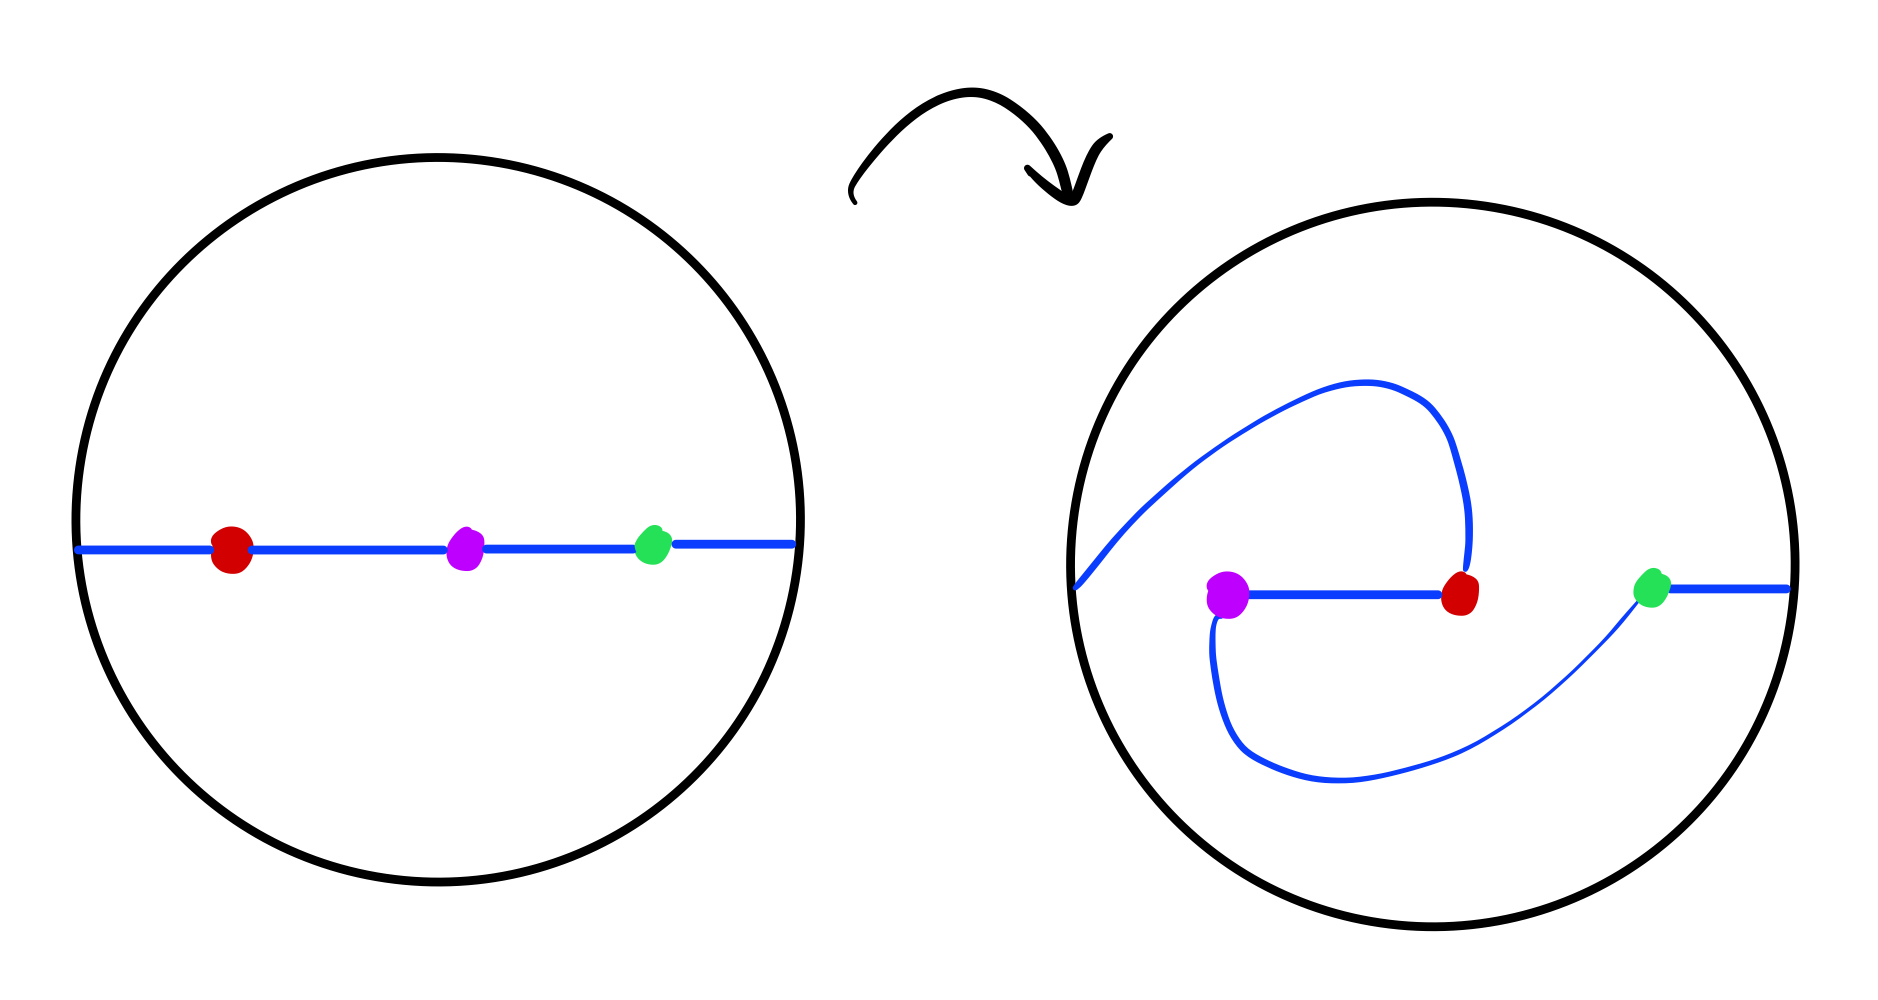
\includegraphics[width=.7\linewidth]{fig6}
\end{figure}\vspace{-1cm}
La permutación representada intercambia los puntos marcados rojo y morado. La curva azul nos sirve para visualizar la acción del homeomorfismo en todo el disco. Decimos que este homeomorfismo es un \textbf{\textit{medio giro}}.

Por el isomorfismo de grupos anterior, concluimos que $\Mod(S_{0,n})$ está generado por una colección de medios giros y una colección de generadores de $\PMod(S_{0,n})$. De hecho,

\begin{teo}[\cite{primer}, teo. 4.9]
	Para $n\geq0$, el grupo $\PMod(S_{0,n})$ está generado por una cantidad finita de giros de Dehn.
\end{teo}

Que a su vez es corolario del teo. 4.6, donde se establece la \textbf{\textit{sucesión exacta de Birman}}. Aunque en el teorema se enuncia de manera más general, nosotros usaremos la restricción a $\Mod(S_{n,g})$):
\[\begin{tikzcd}
	1\arrow[r]&\pi_1(S_{g,n})\arrow[r]&\PMod(S_{g,n+1})\arrow[r]&\PMod(S_{g,n})\arrow[r]&1
\end{tikzcd}\]
Iterando esta sucesión partiendo de que $\PMod(S_{0,n})=1$ para $n\leq3$ y conociendo los grupos fundamentales de cada esfera con puntos marcados, se concluye que $\PMod(S_{0,n})$ es una extensión iterada de grupos libres. Por ejemplo, $\PMod(S_{0,5})\approx F_2\ltimes F_3$.

Recordemos que si la sucesión exacta
\[\begin{tikzcd}
	1\arrow[r]&K\arrow[r]&G\arrow[r]&Q\arrow[r]&1
\end{tikzcd}\]
se \textbf{\textit{escinde}}, $G\approx Q\ltimes K$ (\cite{Rotman}, teo. 10.8). En el caso de $\PMod(S_{0,5})$, la sucesión se escinde porque el grupo de la derecha es libre (\cite{hatcher}, p. 148). (La sucesión exacta de Birman no siempre se escinde).

Finalmente observemos cómo funciona la flecha que sale del grupo fundamental. Se trata del mapeo que Margalit llama $\mathcal{P}ush$, donde un representante de un elemento en el grupo fundamental está asociado a un producto de dos giros de Dehn en el mapping class group como sigue. A una curva $\alpha$ le asociamos dos curvas $a$ y $b$ que están un poco a la izquierda y a la derecha de $\alpha$.


Si $T_a$ y $T_b$ son los giros de Dehn respecto a $a$ y $b$,
\[\alpha\xmapsto{\mathcal{P}ush}T_aT_b^{-1}\]
\begin{figure}[H]
	\centering
	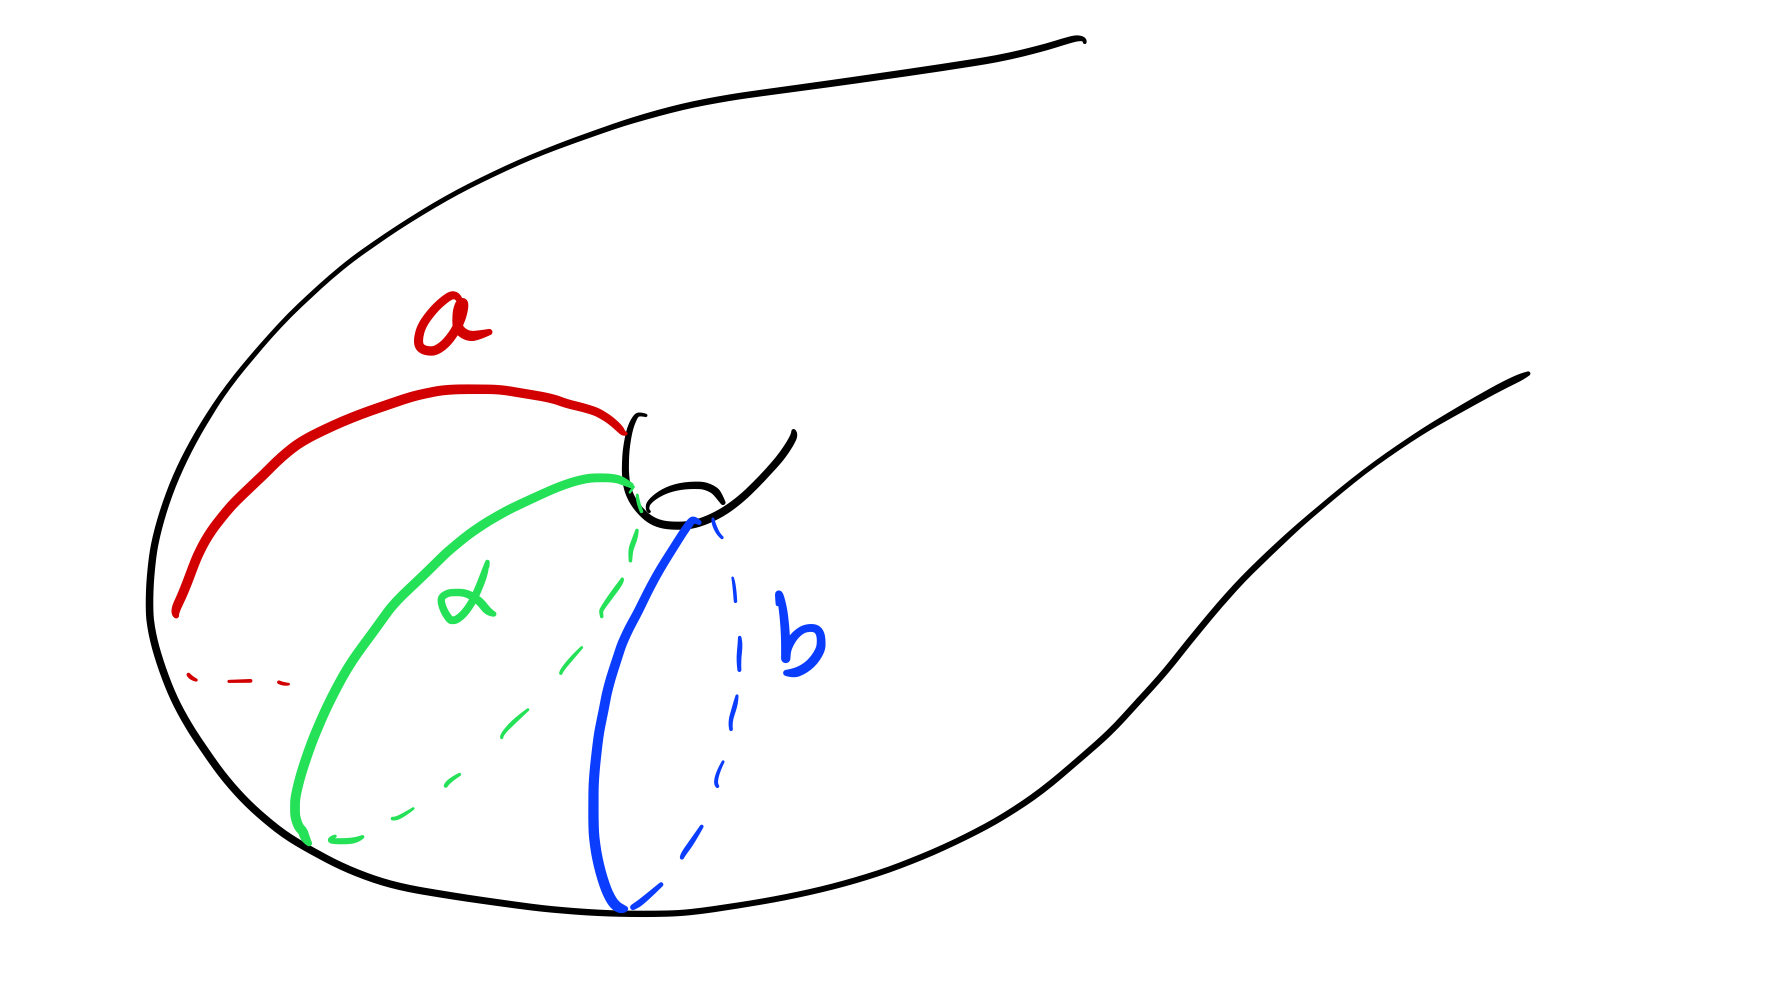
\includegraphics[width=.7\linewidth]{fig10}
\end{figure}

En conclusión, $\PMod(S_{0,n})$ es una extensión de grupos libres, cuyos generadores son productos de dos giros de Dehn, y $\Mod(S_{0,n})$ está generado por esos mismos generadores y una colección de medios giros.




\section{Una presentación de $\Mod(S_2)$}
Ahora comenzamos con nuestro tema. Sabemos que la involución hiperelíptica $\iota$ induce un cubriente $S_g\to S^2_{0,2g+2}$, es decir, de la superficie de género $g$ en la esfera con $2g+2$ puntos marcados. Primero observemos que el grupo de transformaciones de deck es $\langle \iota\rangle$, que es soluble. Como $S_2$ es una superficie hiperbólica, por el teorema de Birman-Hilden y sus equivalencias tenemos que
\[\SMod(S_g)/\langle\iota\rangle\cong\LMod(S_{0,2g+2})\]
Para el caso de género 2, resulta ser que
\[\SMod(S_2)=\Mod(S_2),\]
es decir, cualquier mapping class de $S_2$ es simétrica respecto a la involución hiperelíptica. Para verlo usamos los generadores de Humphries, de que $\Mod(S_2)$ está generado por los giros de Dehn respecto a las siguientes cinco curvas (\cite{primer}, p. 89):
\begin{figure}[H]
	\centering
	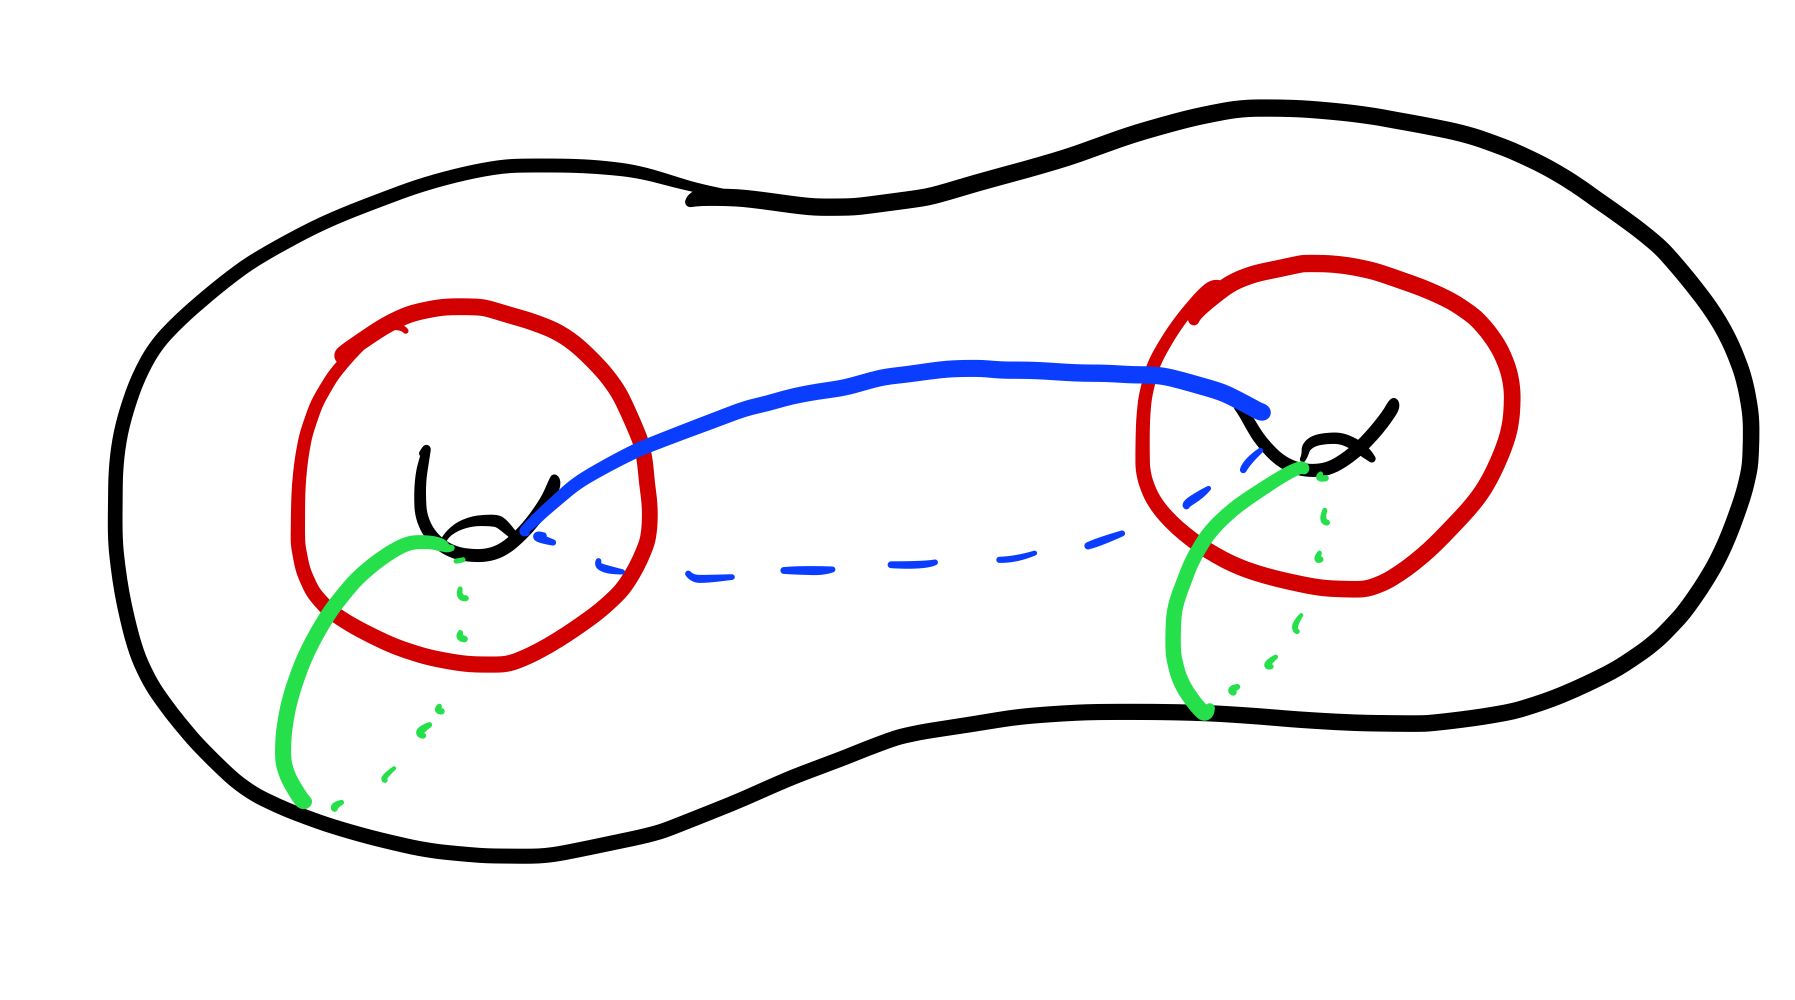
\includegraphics[width=0.7\linewidth]{fig1}
\end{figure}
Reacomodando ligeramente las curvas verde y azul, observamos que de hecho la involución hiperelíptica las fija:
\begin{figure}[H]
	\centering
	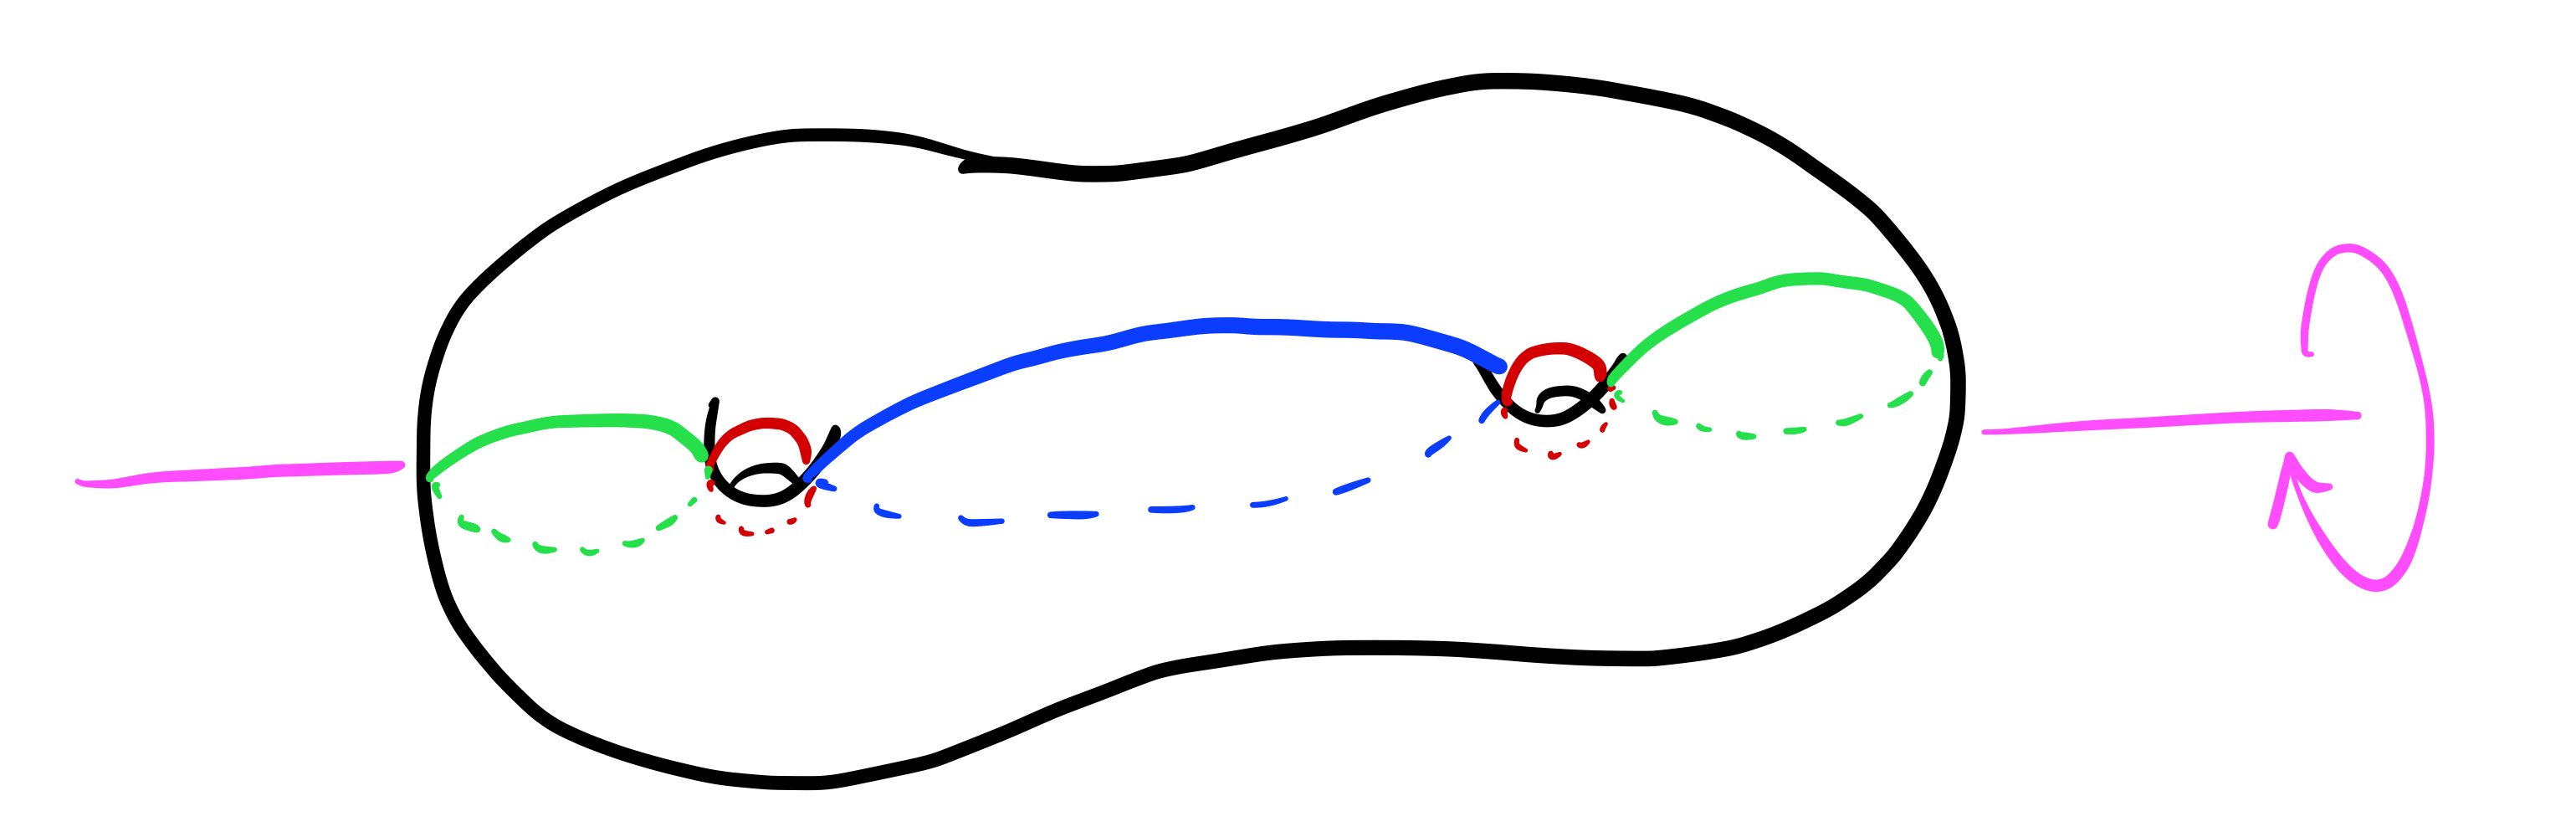
\includegraphics[width=\linewidth]{fig2}
\end{figure}
De aquí se sigue que estos giros de Dehn mandan fibras en fibras. Veamos por qué.

Tomemos el ejemplo del giro de Dehn respecto a la curva verde más a la izquierda. Mostrando dos curvas de referencia morada y naranja, este giro actúa así:
\begin{figure}[H]
	\centering
	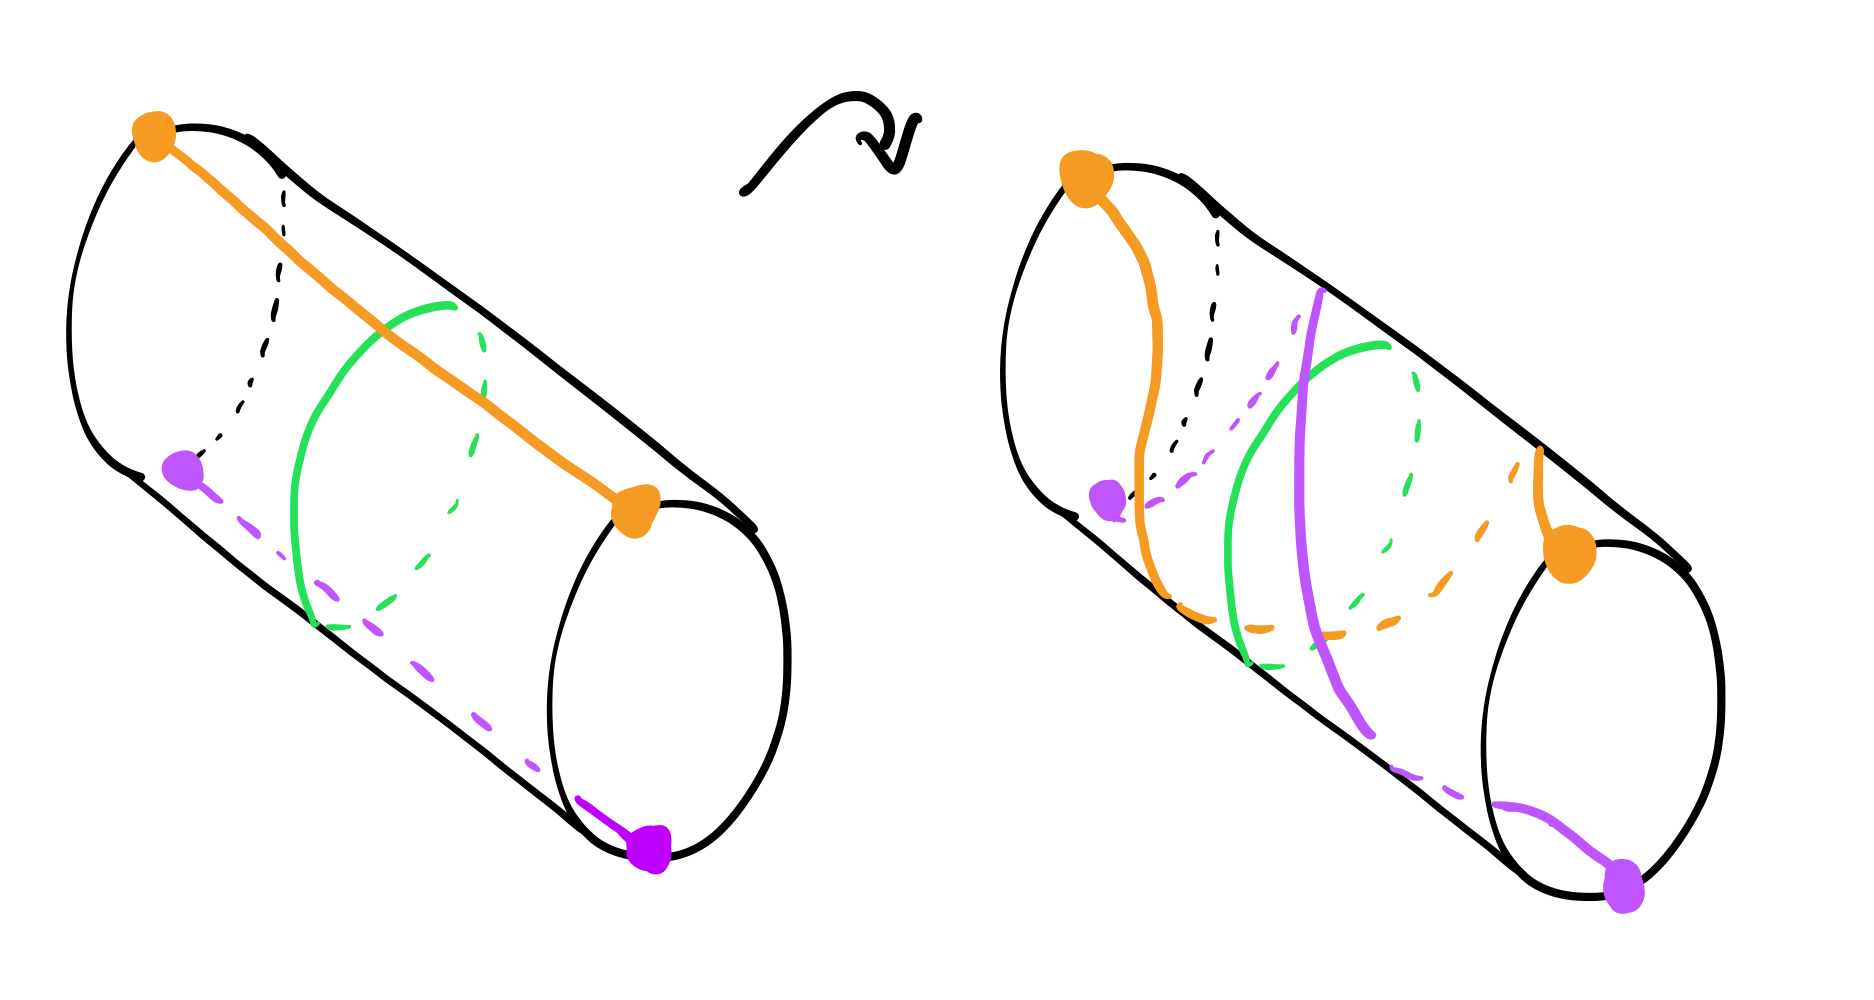
\includegraphics[width=\linewidth]{fig3}
\end{figure}

Ahora tomemos la fibra de algún punto en el cociente, es decir, dos puntos que se identifican mediante la involución hiperéliptica. Suponiendo que la curva azul y la verde están a la altura máxima y mínima de $S_2$, respectivamente, una fibra y su imagen bajo el giro de Dehn se ven así:

\begin{figure}[H]
	\centering
	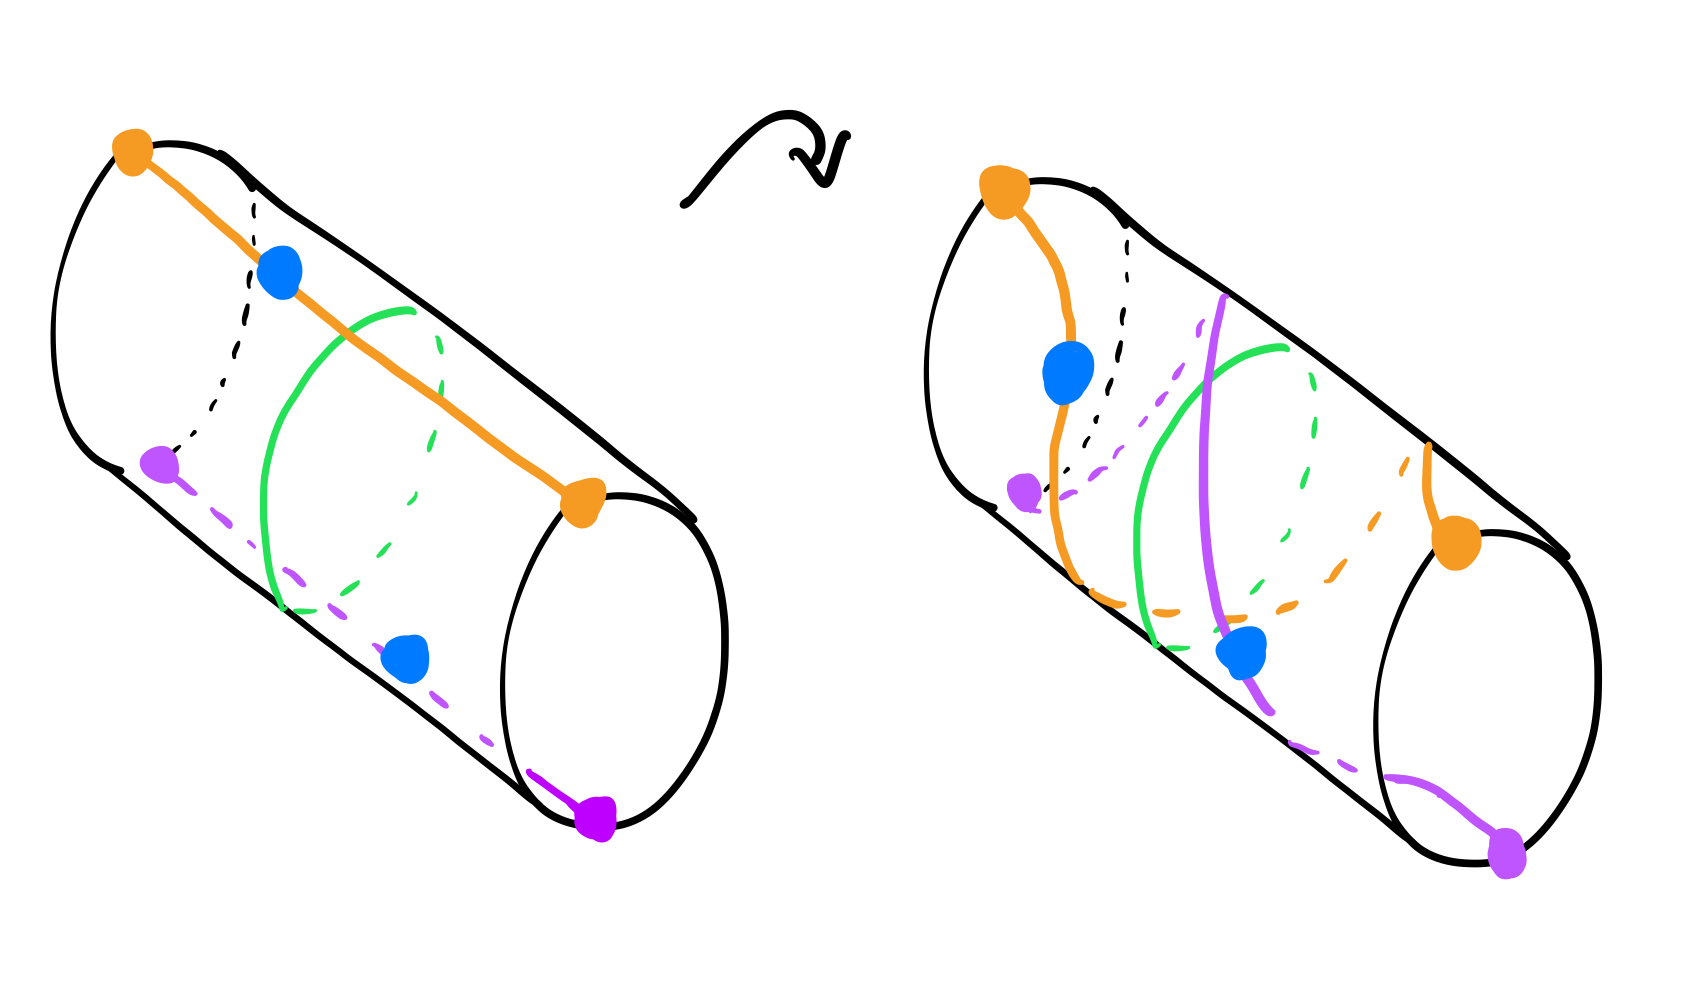
\includegraphics[width=\linewidth]{fig4}
\end{figure}

¿Realmente la pareja de puntos en la figura de la derecha son una fibra?

\begin{figure}[H]
	\centering
	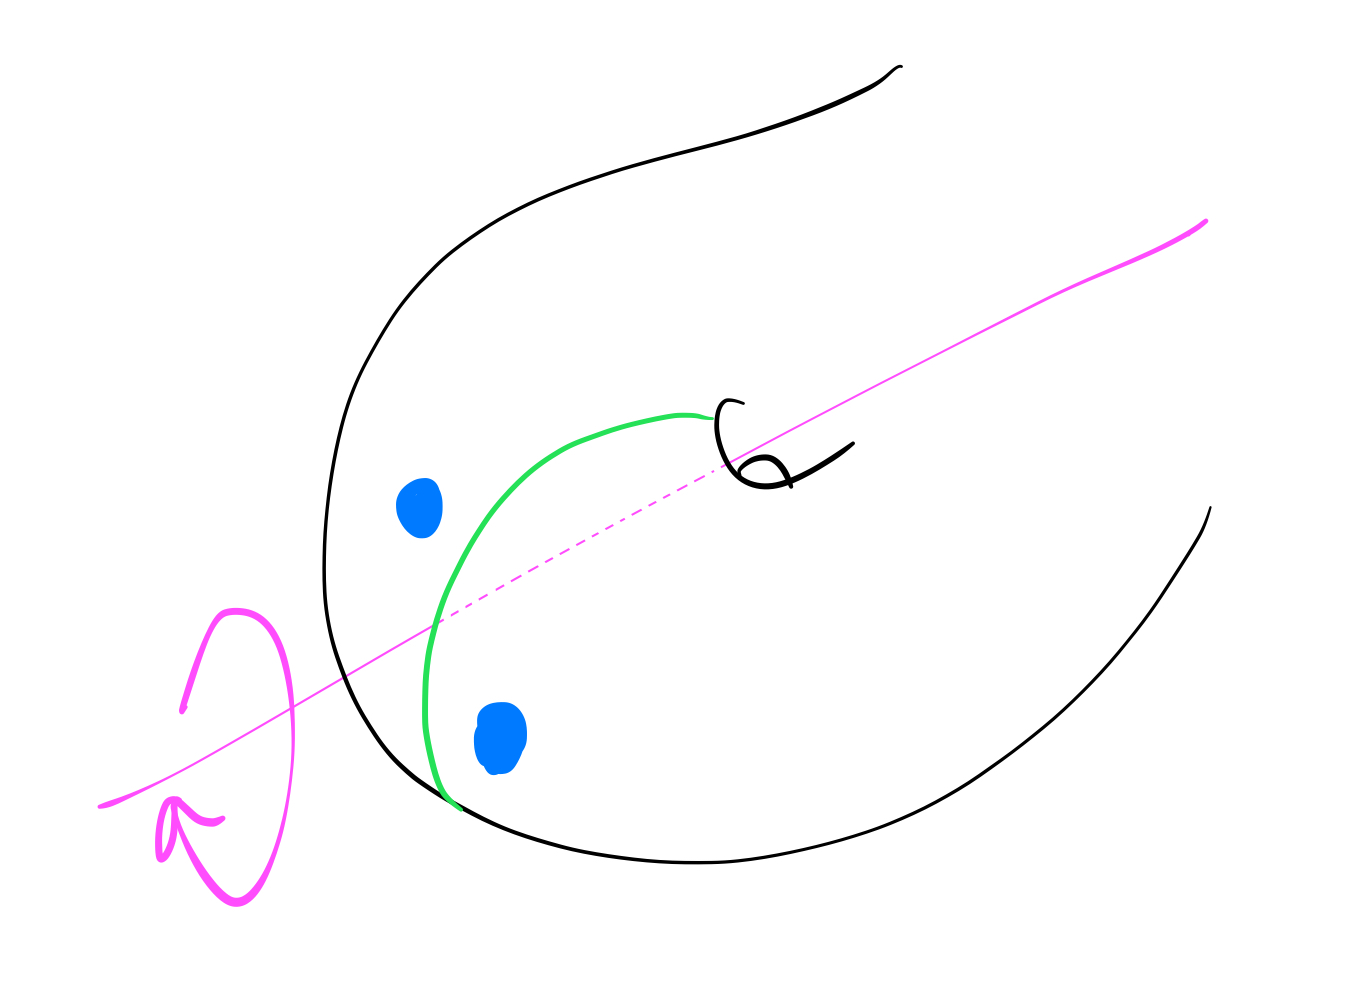
\includegraphics[width=.7\linewidth]{fig5}
	\caption*{¡Sí!}
\end{figure}


Esto implica que
\[\Mod(S_2)/\langle\iota\rangle\cong\LMod(S_{0,6}).\]
Además, resulta que (y en general, para cualquier $S_{0,2g+2}$ con la involución hiperelíptica):
\[\LMod(S_{0,6})\cong\Mod(S_{0,6}).\]
Para verlo, recordemos que $\Mod(S_{0,6})$ está generado por una colección de generadores de $\PMod(S_{0,6})$ y una colección de medios giros.
\iffalse Primero veamos qué pasa con los generadores de $\PMod(S_{0,6})$. Como son funciones que fijan los puntos marcados, podemos considerarlos como funciones del cubriente no ramificado asociado y aplicar el criterio de levantamiento de funciones. Si $T_aT_b^{-1}$ es uno de estos generadores, tenemos el diagrama
\[\begin{tikzcd}
	&&S_{2,6}\arrow[d,"p"]\\
	S_{2,6}\arrow[urr,dashed,"\widetilde{pT_aT_b^{-1}}"]\arrow[r,swap,"p"]&S_{0,6}\arrow[r,swap,"T_aT_b^{-1}"]&S_{0,6}
\end{tikzcd}\]
donde el levantamiento existe si
\[(T_aT_b^{-1}p)_*\pi_1(S_{2,6})\subseteq p_*\pi_1(S_{2,6}),\]
Por funtorialidad tenemos que \[(T_aT_b^{-1}p)_*\pi_1(S_{2,6})=(T_aT_b^{-1})_*p_*\pi_1(S_{2,6})\overset{?}{\subseteq}p_*\pi_1(S_{2,6})\]
De acuerdo a \href{https://math.stackexchange.com/questions/1874/presentation-of-the-fundamental-group-of-a-manifold-minus-some-points}{esta fuente}, el grupo fundamental de una superficie de género $g$ con $r$ puntos marcados es el grupo libre de $2g+r-1$ elementos. Así, $\pi_1(S_{2,6})\approx F_9$ y $\pi_1(S_{0,6})\approx F_6$. No es evidente qué son $p_*\pi_1(S_2)$ y $(T_aT_b^{-1})p_*\pi_1(S_2)$. Tratemos de argumentarlo visualmente.
\fi
Los generadores de $\PMod(S_{0,6})$ son productos de giros de Dehn asociados a curvas que representan los generadores del grupo fundamental.

En la siguiente figura mostramos nuestro cubriente con los seis puntos marcados. Las curvas azules representan los generadores del grupo fundamental de $S_{0,6}$ y sus levantamientos en $S_2$:
\begin{figure}[H]
	\centering
	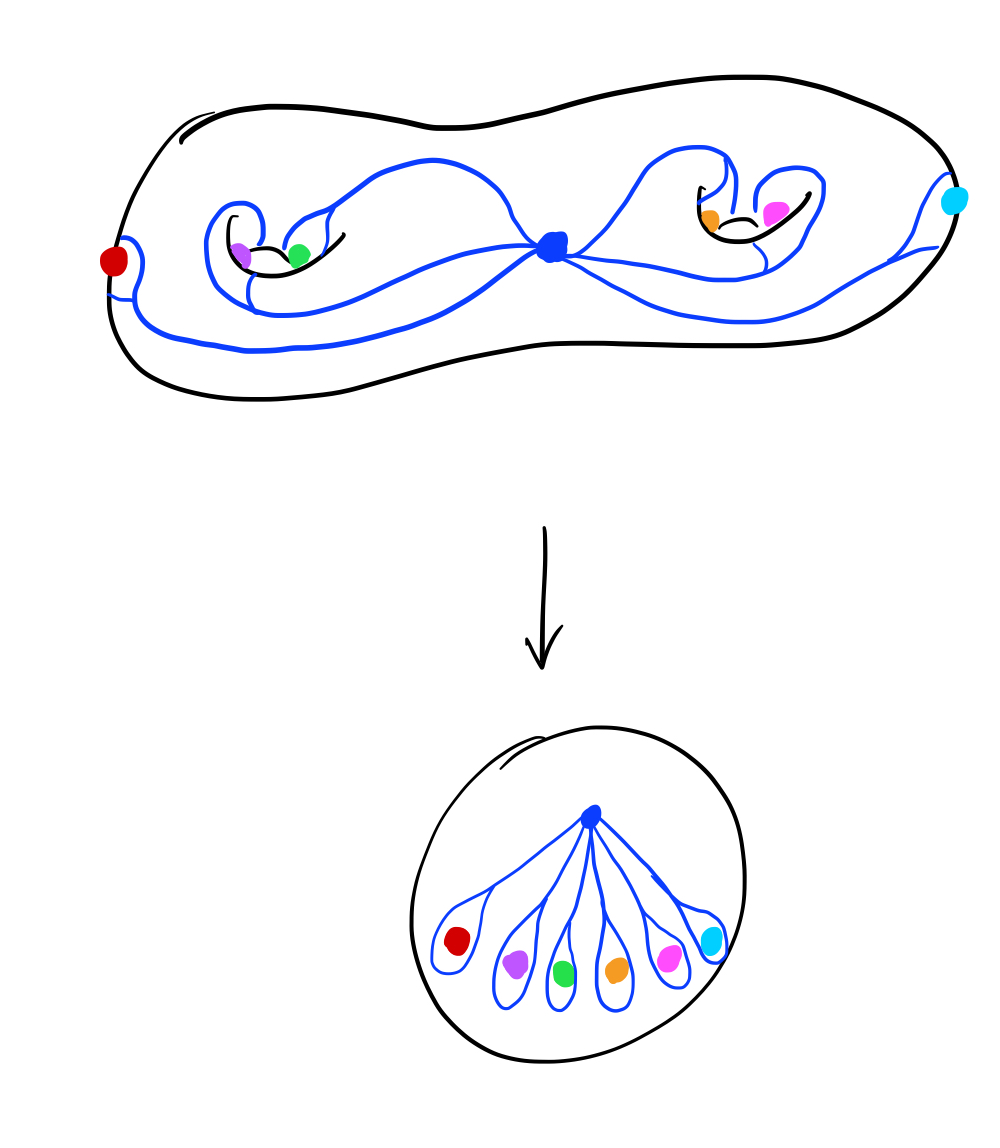
\includegraphics[width=.7\linewidth]{fig21}
\end{figure}
Podemos ver que las curvas azules en $S_2$ son contraibles.

Ahora veamos qué pasa con los medios giros.
\clearpage
¿Cómo se ven estos medios giros en el caso de nuestro cubriente?
\begin{figure}[H]
	\centering
	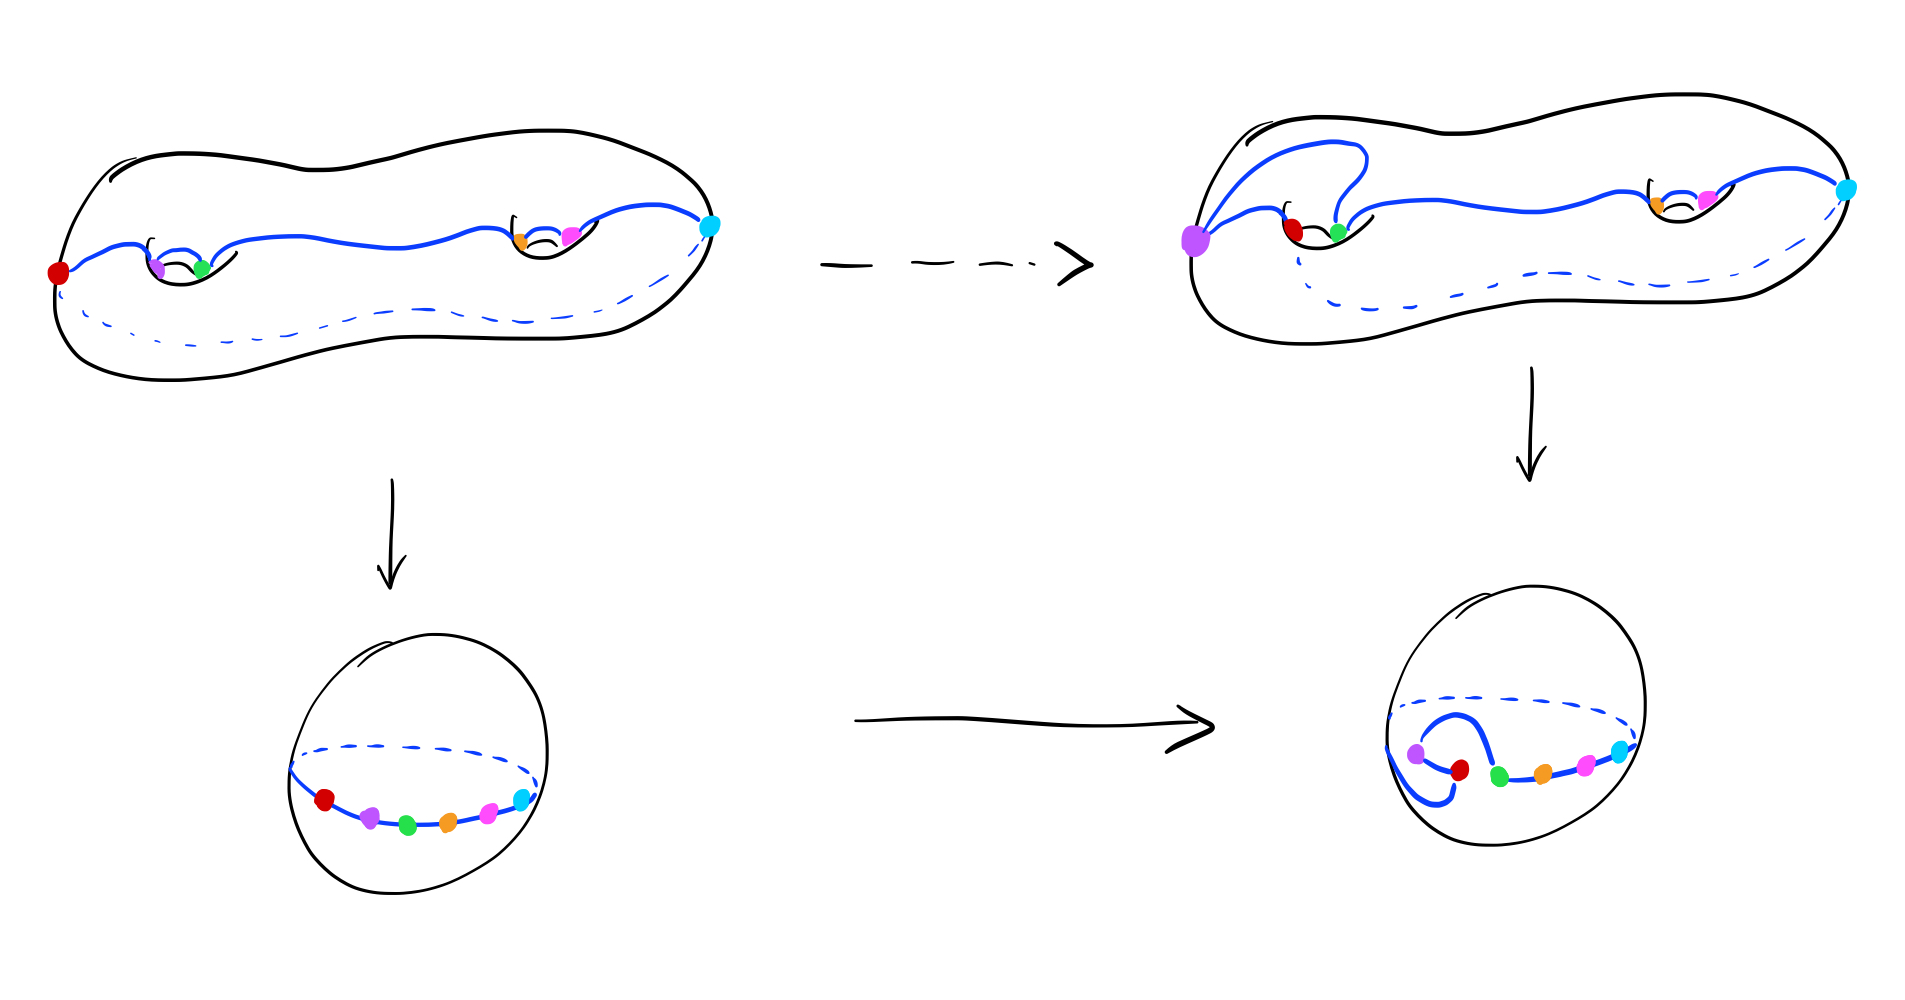
\includegraphics[width=\linewidth]{fig7}
\end{figure}
\vspace{-1cm}
En esta figura mostramos un ejemplo que permuta los puntos rojo y morado. La observación clave es que los levantamientos de estos medios-giros (la flecha punteada en la figura) de hecho son giros de Dehn. Podemos visualizar este ejemplo de la siguiente manera:
\begin{figure}[H]
	\centering
	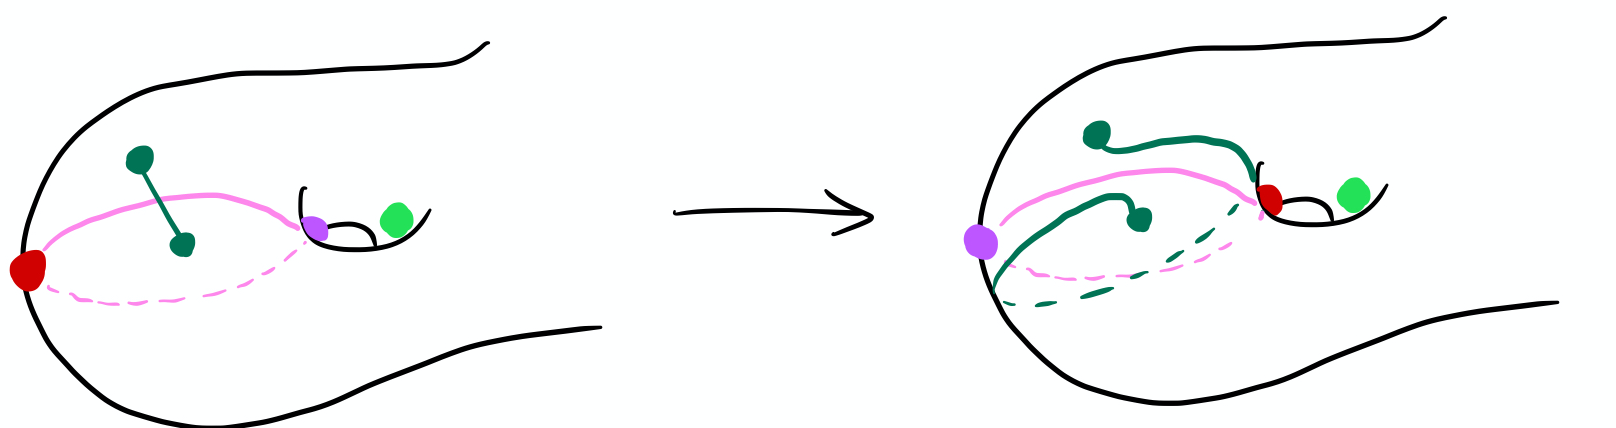
\includegraphics[width=\linewidth]{fig8}
	\caption*{\textit{El giro de Dehn respecto a la curva rosa mostrando una curva verde oscuro de referencia.}}
\end{figure}
\begin{figure}[H]
	\centering
	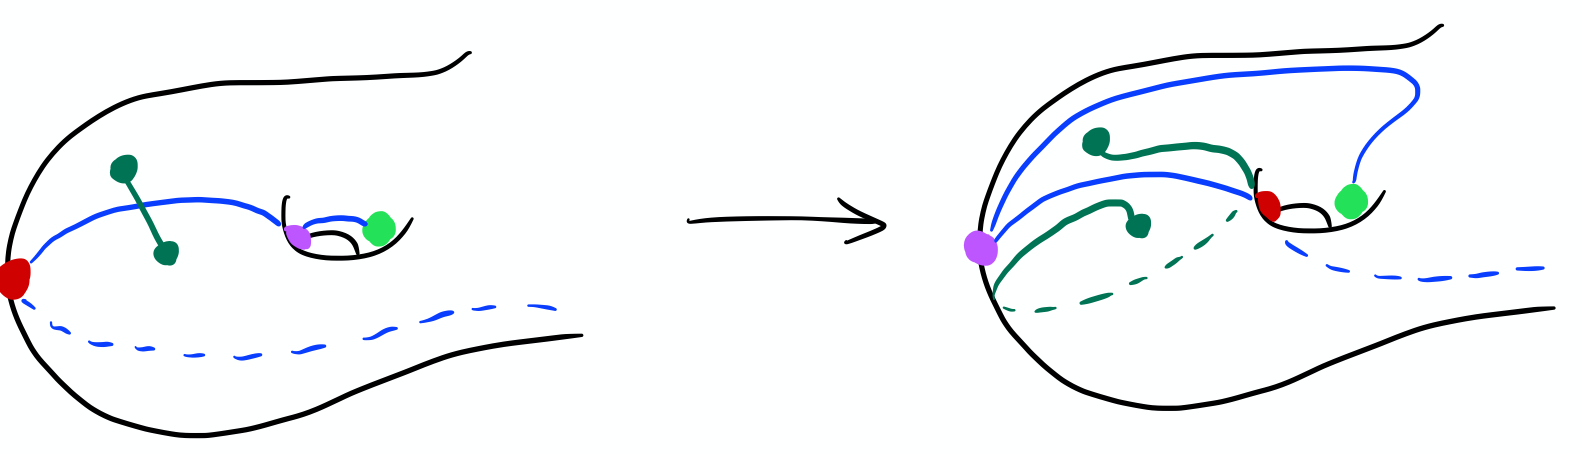
\includegraphics[width=\linewidth]{fig9}
	\caption*{\textit{¡El giro de Dehn hace lo mismo que el levantamiento del medio giro!}}
\end{figure}

Finalmente concluimos que
\[\Mod(S_2)/\langle\iota\rangle\approx\Mod(S_{0,6})\]

Los generadores de $\Mod(S_{0,6})$ fueron encontrados por Magnus, y de ellos Birman y Hilden encontraron la siguiente presentación para $\Mod(S_2)$ dada en términos de los generadores de Humphries $T_1$ a $T_5$:
\begin{align*}
	[T_i,T_j]=1&\qquad \text{para }|i-j|\geq2\\
	T_iT_{i+1}T_i=T_{i+1}T_iT_{i+1}&\qquad\text{para }1\leq i \leq 4\\
	(T_1T_2T_3T_4T_5)^6=1&\\
	(T_1T_2T_3T_4T_5T_5T_4T_3T_2T_1)^2=1&\\
	[T_1T_2T_3T_4T_5T_5T_4T_3T_2T_1,T_1]=1&
\end{align*}

Las primeras dos son las relaciones del grupo de trenzas $B_6$, la siguiente describe el kernel de $B_6\to\Mod(S_{0,6})$, y las últimas dos corresponden a la involución hiperelíptica, que es $T_1T_2T_3T_4T_5T_5T_4T_3T_2T_1$.

El método para obtener esta presentación se puede encontrar en \S4 \cite{BirmanHilden2}.

\section{Generalización para $\SMod(S_g)$}
Como recordatorio, dados $p_1,\ldots,p_n\in\C$, el \textbf{\textit{grupo de trenzas}} $B_n$ consiste de las clases de isotopía de $n$ caminos $f_i:[0,1]\to\C\times[0,1]$ tales que $f_i[0,1]$ son disjuntos, $f_i(0)=p_i$, $f_i(1)=p_{\bar{f}(i)}$ y $f_i(t)\in\C\times\{t\}$ para alguna permutación de $n$ elementos $\bar{f}$. Este grupo está generado por $n-1$ elementos que satisfacen las siguientes relaciones (\cite{primer}, p. 246):
\begin{align*}
	\sigma_i\sigma_j&=\sigma_j\sigma_i\quad \;\;\;\qquad\quad\text{para }|i-j|\geq2\\
	\sigma_i\sigma_{i+1}\sigma_i&=\sigma_{i+1}\sigma_i\sigma_{i+1}\qquad\text{para toda }i
\end{align*}

En \cite{birman-isotopies} tenemos la siguiente generalización para $\SMod(S_{g})$. Dados los generadores $t_1,\ldots,t_{n-1}$, las relaciones son
\begin{align*}
	[t_i,t_j]=1&\qquad \text{para }i,j=1,\ldots,n-1\text{ tales que }|i-j|\geq2\\
	t_it_{i+1}t_i=t_{i+1}t_it_{i+1}&\qquad\text{para }i=1,\ldots,n-2\\
	(t_1t_2\ldots t_{n-1})^n=1&\\
	(t_1t_2\ldots t_{n-1}t_{n-1}\ldots t_2t_1)^k=1&\\
	[t_1t_2\ldots t_{n-1}t_{n-1}\ldots t_2t_1,t_1]=1&
\end{align*}
donde, en casos más generales, $2g=(k-1)(n-2)$. Si $n=2g+2$ es la cantidad de puntos marcados, tenemos simplemente que $k=2$.

Si $D_n$ es el disco $D^2$ con $n$ puntos marcados, tenemos el siguiente isomorfismo:
\[B_n\approx \Mod(D_n)\]
La correspondencia está dada como sigue. Un elemento de $\Mod(D_n)$ puede ser pensado como un homeomorfismo del disco en sí mismo. Sabemos que $\Mod(D^2)\approx1$, de forma que hay una isotopía con la identidad. En cada momento de la isotopía, los de puntos marcados se mueven en el interior del disco y vuelven al punto inicial, de manera que tenemos una trenza.
\begin{figure}[H]
	\centering
	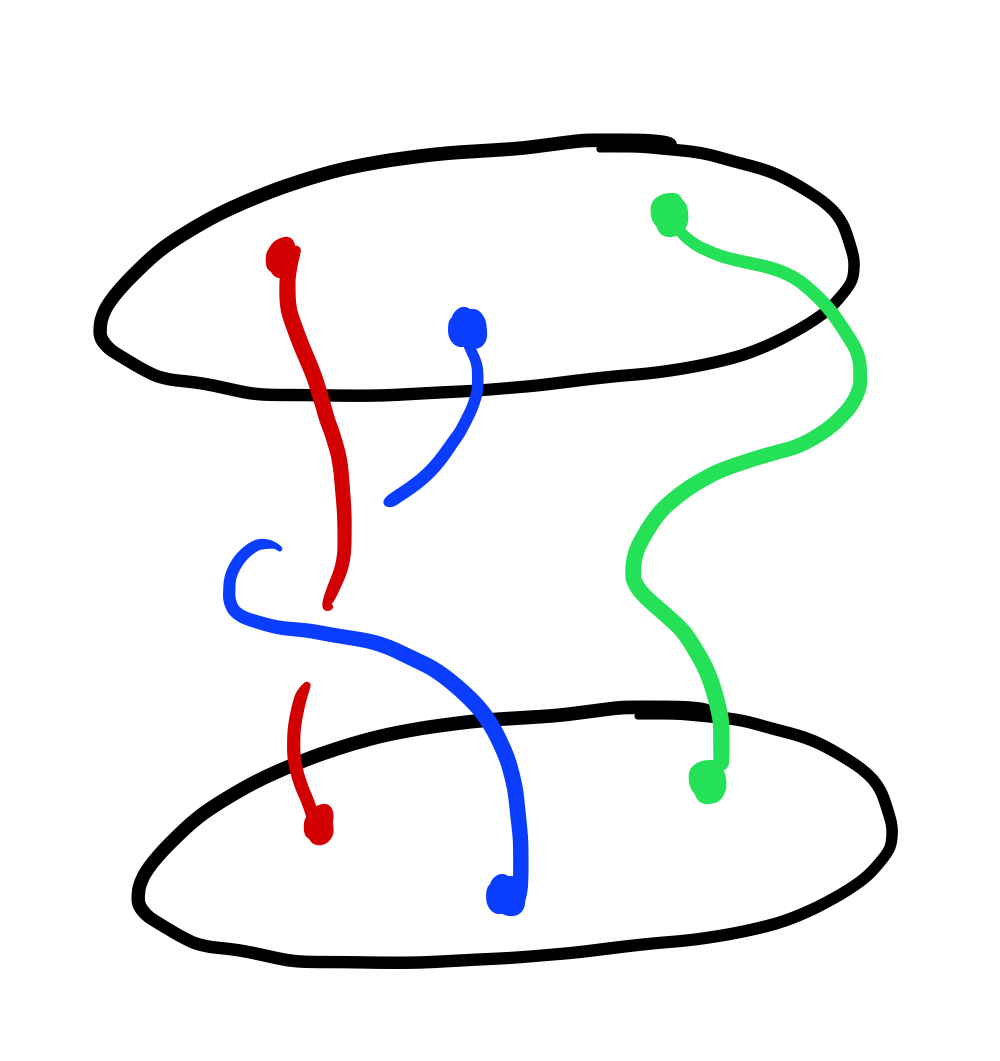
\includegraphics[width=0.4\linewidth]{fig27}
\end{figure}
La demostración de que esta correspondencia es un isomorfismo se obtiene de una generalización de la sucesión exacta de Birman (\cite{primer}, teo. 9.1)

Por último mencionamos que para la superficie de género $g$ con una componente frontera, se tiene el siguiente resultado (\cite{primer}, teo. 9.2):
\[\SMod(S^1_g)\approx B_{2g+1}\]
En este caso el cociente bajo la involución hiperelíptica es un disco con $2g+1$ puntos marcados:
\begin{figure}[H]
	\centering
	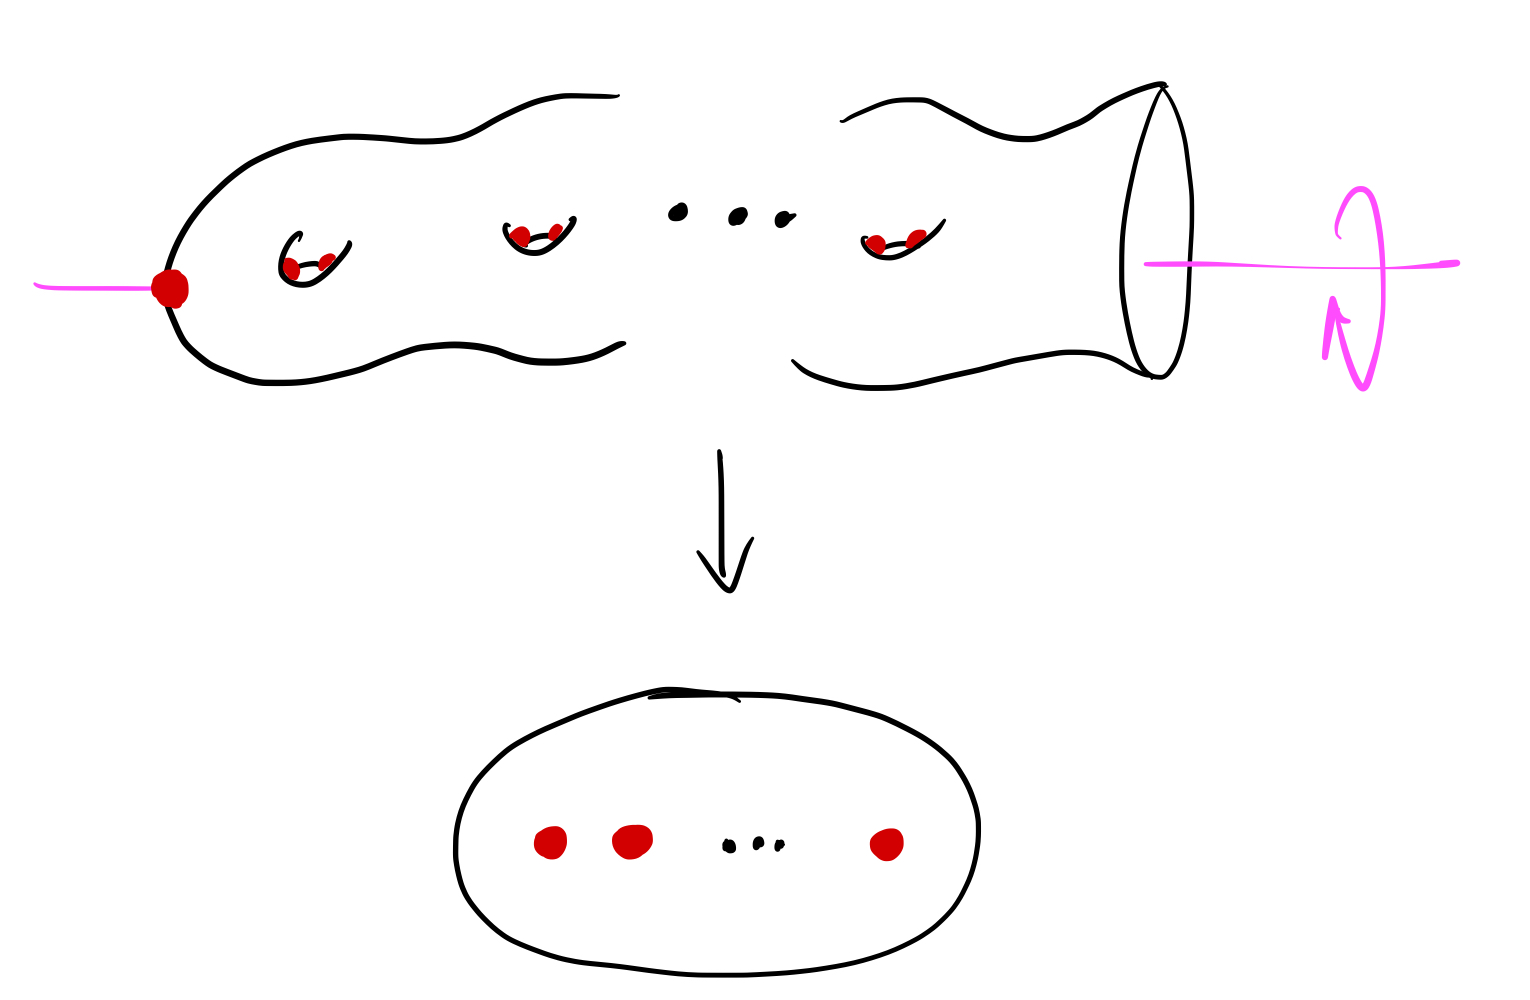
\includegraphics[width=\linewidth]{fig25}
\end{figure}
	Por el teorema de Birman-Hilden, las homotopías en $S_g^1$ pasan al cociente, y además los homomorfismos del disco punteado son levantables, así que
\[\SMod(S^1_g)\approx\Mod(D_{2g+1}) \approx B_{2g+1}\]


\section{Aplicaciones}
\subsection{La signatura de una 4-variedad}

La \textbf{\textit{signatura de una 4-variedad}} $M$ conexa y orientada es la signatura de la forma cuadrática inducida por el producto copa en $H^2(M;\R)$ como sigue. Recordemos que el producto copa es un operador
\begin{align*}
	\smile:H^k(M;\R)\times H^{n-k}(M;\R)\to H^{n}(M;\R)
\end{align*}
en los grupos de cohomología. Como los $n$-cociclos son homomorfismos $H_n(M;\R)\to\R$, podemos calcular
\[\alpha\smile\beta([M])\]
donde $[M]$ es la clase fundamental dada por la orientación de $M$.

El mapeo resultante es el \textbf{\textit{apareamiento del producto copa}},
\begin{align*}
	\smile:H^k(M;\R)\times H^{n-k}(M;\R)\to \R
\end{align*}
 que es un operador no degenerado en el sentido de que $\alpha\smile\beta=0$ para toda $\beta\in H^{n-k}(M;\R)$ implica $\alpha=0$, y análogamente para $\beta$. Este tipo de operadores están en biyección con las \textbf{\textit{formas bilineales simétricas}}.
 
 Por la \textbf{\textit{ley de inercia de Sylvester}}, la cantidad de números positivos, negativos y cero en la matriz diagonalizada asociada a una forma bilineal simétrica es invariante bajo cambios de base. La \textbf{\textit{signatura de una forma cuadrática}} $Q$ es $\sigma(Q)=n_++n_-$ donde cualquier matriz diagonal que represente a $Q$ tiene $n_+$ entradas positivas y $n_-$ entradas negativas. La \textbf{\textit{signatura de una 4-variedad}} $M$ es la signatura del operador $\smile$ que hemos definido.
 
 Interesantemente (ver \cite{Atiyah}), 
 \[\operatorname{Sign}(X\times Y)=\operatorname{Sign}(X)\operatorname{Sign}(Y)\]
 definiendo la signatura $\operatorname{Sign}(X)=0$ si la dimensión de $X$ no es divisible entre 4.
 
 Un \textbf{\textit{haz fibrado}} en un espacio $E$ con base $B$ y fibra $F$ es una proyección $p:E\to B$ tal que para cada $p\in B$ hay una vecindad $U$ y un homeomorfismo $h:p^{-1}(U)\to U\times F$ tal que el siguiente diagrama conmuta:
 \[\begin{tikzcd}
 	p^{-1}(U)\arrow[r,"h"]\arrow[d,"p",swap]&U\times F\arrow[ld]\\
 	U
 \end{tikzcd}\]
 donde la flecha de la derecha es la proyección al primer factor. Se trata de una correspondencia que a cada punto de $U$ asocia una copia de $F$. En el caso del \textbf{\textit{haz tangente}}, a cada punto asociamos su espacio tangente.
 
 En la fórmula multiplicativa de la signatura de una 4-variedad, es posible reemplazar $X\times Y$ por un haz fibrado con base $X$ y fibra $Y$ bajo ciertas condiciones. Un contraejemplo está dado por un \textbf{\textit{haz de superficies}} en una superficie, un haz fibrado cuya base y fibra son superficies, que tiene estructura de 4-variedad.
 
 En este contexto, Meyer mostró que si un haz de superficies sobre una superficie tiene \textbf{\textit{monodromía}} en $\SMod(S_g)$, entonces la signatura de la 4-variedad que resulta es cero. La monodromía de un \textbf{\textit{mapping torus}} es justamente la función de pegado.
 
 %La \textbf{\textit{monodromía}} es un grupo que se asocia a los levantamientos de caminos en un cubriente de superficies de Riemann \cite{diez}. Intuitivamente, para un cubriente de grado $d$, el levantamiento de un lazo en el espacio base induce una permutación de $d$ elementos dada por el punto inicial y el punto final. Así, el grupo fundamental del espacio base menos los puntos de ramificación tiene una representación en el grupo simétrico de $d$ elementos.

\iffalse
Un \textbf{\textit{haz de superficies}} es una función que a cada punto de una variedad asigna una superficie. Cuando la variedad también es una superficie, el haz tiene estructura de 4-variedad (\cite{hatcher}, p. 377). \textcolor{cyan}{Grupo estrucutral, clasificante, clasificar haces complejos, clases de Chern, Stifel-Withney, Pont., . El grupo estructural es el grupo de difeomorfismos de la superficie. Queremos estudiar el espacio clasificante del grupo de difeomorfismos de la superficies,. Cuando al superficie es hiperbólica el espacio aclasficcante tiene el mismo tipo de homotopía, tiene la misma cohomología que el grupo modular así que conociendo la cohomología podemos conocer clases características de haces de superficies. Si el haz de superficies con el que comienzo, cae en SMod en contes la 4-variedad tiene signatura 0.}

\textcolor{magenta}{¿Cuál es el mapping torus? A pues es un haz de superficies. Pegar las tapas. ¿Qué tipo de geometría le damos a esta 3-variedad?}

La \textbf{\textit{signatura de una 4-variedad}} $M$ conexa y orientada es la signatura de la forma cuadrática inducida por el producto copa en $H^2(M;\R)$. Por la paridad de la dimensión, el producto copa es simétrico en este grado (en general es antisimétrico) y, por dualidad de Poincaré, su contradominio $H^4(M;\R)$ es isomorfo a $H^0(M;\R)\approx\R$ y el apareamiento es no degenerado (así que la forma cuadrática correspondiente es no degenerada) \cite{wiki}. \textcolor{cyan}{Muy bonito y explicado.}

Recordemos que la \textbf{\textit{signatura de una forma cuadrática}} $Q$ es $\sigma(Q)=n_++n_-$ donde cualquier matriz diagonal que represente a $Q$ tiene $n_+$ entradas positivas y $n_-$ entradas negativas.

La \textbf{\textit{monodromía}} es un grupo que se asocia a los levantamientos de caminos en un cubriente de superficies de Riemann \cite{diez}. Intuitivamente, para un cubriente de grado $d$, el levantamiento de un lazo en el espacio base induce una permutación de $d$ elementos dada por el punto inicial y el punto final. Así, el grupo fundamental del espacio base menos los puntos de ramificación tiene una representación en el grupo simétrico de $d$ elementos. \textcolor{magenta}{¿Cómo es la monodromía de un haz de superficies?}\fi

\subsection{Cohomología en dimensiones bajas de $\SMod(S_g)$}
En \cite{kawazumi}, Kawazumi estudia \textbf{\textit{curvas hiperelípticas}} en $\C^2$, que son superficies de Riemann definidas mediante polinomios de la forma
\[w^2=\prod_{i=1}^{2g+2}(z-a_i),\qquad \text{ con }a_i\neq a_j \text{ cuando }i\neq j\]
(es decir, los factores tienen multiplicidad 1) (ver \cite{diez}). Estas superficies admiten \textbf{\textit{involuciones hiperelípticas}}, que son funciones de la forma $(z,w)\mapsto (z,-w)$.

El objetivo de su artículo es, dada una involución hiperelíptica $\iota$, estudiar la cohomología del centralizador de $\iota$ en el mapping class group, es decir, $\SMod(S_g):=\Delta_g$.

Se construyen las siguientes dos sucesiones exactas:
\[\begin{tikzcd}[column sep=small,row sep=tiny]
	\cdots\arrow[r]&H^{q+3}(\Delta_{g,1})\arrow[r]&H^q(\Delta_g)\arrow[r]&H^{q+4}(\Delta_g)\arrow[r]&H^{q+4}(\Delta_{g,1})\arrow[r]&\cdots
	\\
	\cdots\arrow[r]&H^{q-2}(B_{2g+1})\arrow[r]&H^q(\Delta_{g,1})\arrow[r]&H^q(B_{2g+2})\arrow[r]&H^{q-1}(B_{2g+1})\arrow[r]&\cdots
\end{tikzcd}\]
donde $\Delta_{g,1}$ es el producto fibrado de $\Delta_1$ con el haz tangente menos la sección cero. Usando las dos sucesiones podemos relacionar $\Delta_g=\SMod(S_g)$ con un grupo de trenzas.

Obtenemos que el primer grupo de homología es
\begin{align*}
	H_1(\Delta_g;\Z)=\begin{cases}
		\Z/2(2g+1),\qquad\text{ si }g\text{ es par}\\
		\Z/4(2g+1),\qquad\text{ si }g\text{ es impar}
	\end{cases}
\end{align*}
y el primer grupo de cohomología sobre un campo de característica $k$,
\begin{align*}
	H^1(\Delta_g;k)=\begin{cases}
		0,\qquad\text{ si }\operatorname{car}k\nmid 2(g-1)(2g+1)\\
		k,\qquad\text{ si }\operatorname{car}k\mid 2(g+1) \text{ y }\operatorname{car}k\nmid 2(g-1)\\
	\end{cases}
\end{align*}
Luego, usando que $H_1(B_n;\Z)=\Z$ y $H^2(B_{2g+2};k)=0$ cuando $\operatorname{car}k\neq2$,
\begin{align*}
	H^2(\Delta_g;k)\cong H^1(\Delta_g;k).
\end{align*}

\iffalse
Para grado tres, si $\operatorname{car}k\neq2$ y $H^2(B_{2g+2};k)=H^3(B_{2g+2};k)=0$, entonces
\[k\cong H^2(B_{})\cong H^3(\Delta_{g,1})\]
es un isomorfismo.

Además, como $H^q(B_n;k)=0$ para $q\geq2$ y $\operatorname{car}k\geq [n/2]$, y se concluye que
\[H^*(\Delta_g;k)=k\]
cuando $\operatorname{car}k=0$ o ($\geq g+2$ y $\neq2g+1$).

%\subsection{Otros resultados}
\begin{itemize}
	\item $\Mod(S_2)$ es lineal, es decir, hay una representación (un homomorfismo inyectivo) de $\Mod(S_2)$ en $\operatorname{GL}_N(\C)$ para alguna $N$. Se demuestra usando el isomorfismo $\Mod(S_2)/\langle\iota\rangle\cong\Mod(S_{0,6})$ y la linealidad de los grupos de trenzas.
	
	\item $\Mod(S_2)$ contiene un subgrupo normal donde todo elemento no trivial es \textbf{\textit{pseudo-Anosov}} (relacionado con foliaciones).
	
	\item Hay una representación de $\Mod(S_2)$ en $GL_5(\Z[t,t^{-1}])$.
\end{itemize}
\fi
\section{Referencias}
\printbibliography[heading=none]

\end{document}